\documentclass{report}
\usepackage[extreme]{savetrees}
\usepackage{wrapfig}
\usepackage{graphicx}
\graphicspath{{./images/}}
\usepackage{amsthm}
\usepackage{siunitx}
\usepackage{url}
\usepackage{subfig}
\usepackage{lscape}
\usepackage{amsmath}
\usepackage{tikz}
\usepackage{mathdots}
\usepackage{epigraph}
\usepackage{yhmath}
\usepackage{cancel}
\usepackage{float}
\usepackage{color}
\usepackage{siunitx}
\usepackage{array}
\usepackage{multirow}
\usepackage{amssymb}
\usepackage{gensymb}
\usepackage{tabularx}
\usepackage{booktabs}
\usetikzlibrary{fadings}
\title{Marketing Training Report}
\author{Tuneer Bhattacherjee\\Employee Id: 514370\\BhattacherjeeT@indianoil.in}
\makeindex
\begin{document}
	\maketitle
	\pagebreak
	\tableofcontents
	\pagebreak
	\chapter{Sanand Bottling Plant}
	\section{Important Terms and Abbreviations}
	\begin{itemize}
		\item OISD= Oil Industry and Safety Directorate
		\item PESO= Petroleum and Explosives Safety Organization
		\item TT= Tanker Trucks
		\item Cavitation = Cavitation is a phenomenon in which rapid changes of pressure in a liquid lead to the formation of small vapor-filled cavities, in places where the pressure is relatively low.When subjected to higher pressure, these cavities, called "bubbles" or "voids", collapse and can generate an intense shock wave. These shock waves can damage pumps/motors.
		\item CFM= Cubic Feet per Minute
		\item SO= State Office
		\item HO= Head Office
		\item DOA= Delegation of Authority
		\item BCW= Blue Collar Workers
		\item VCB= Vacuum Circuit Breaker
		\item ACB= Air Circuit Breaker
		\item EB= Electricity Board
		\item T/F= Transformer
		\item CT= Current Transformer
		\item PT= Potential Transformer
		\item CB= Circuit Breaker
		\item SFU= Switch Fuse Unit (See Fig \ref{sfu})
		\item EP= Earthing Pit
		\item TLV= Threshold Limit Value
		\item LEL= Lower Explosive Limit
		\item UEL= Upper Explosive Limit
		\item BA= Breathing Apparatus
		\item STEL= Short Term Exposure Level
	\end{itemize}
	\section{Sanand Bottling Plant - Day 1 (13.08.2019)}
	
	\subsection{Introduction to Sanand LPG Bottling Plant - Salient Points}
	\textit{Faculty: Shri. Joydev Ojha, DGM(P), Sanand BP}
	\begin{itemize}
		\item Due to low land prices and government push, this particular bottling plant has much more space than what is required under the OISD guidelines.
		\item In addition to that, there is a 66 acre buffer area which is not required anymore according to the latest OISD guidelines so, the plant "occupier" or location in charge Shri. Joydev Ojha, DGM(P) has decided to utilize it to benefit the corporation in the following ways:-
		\begin{itemize}
			\item A 8MW solar plant was established in the buffer area which generates about Rs.3 lacs of electricity per day, part of which is used up by the factory and part is distributed to other IOCL facilities via the grid. It is important to note that according to the some regulations in the Gujrat solar power consumption policy, IOCL at max can only generate 50\% of their net electricity demand if they wish to stay on grid and share their power with other IOCL facilities using the same. This facility covers 66 acre of the buffer area. 
			
			\item  A 2 acre lube storage facility (CFA). It is important to note here that lube being a high flashpoint product is an ``excluded product''. Therefore, storing it in buffer areas donot raise any safety concerns.
			
			\item 4 acres are being delegated to the pipelines division to facilitate the Kandla-Gorakhpur pipeline.
			
			
		\end{itemize}
		\item Product is sourced into the bottling plant using approximately 100 LPG TTs of 18-20 MTs from the following sources -
		\begin{itemize}
			\item Kandla port
			\item Pipawa port
			\item Varoda refinery
			\item Reliance refinery, Jamanagar
			\item Essar refinery, Jamnagar etc.
		\end{itemize}
	
		\item There are 8 TLDs which takes about 3-4 hours to completely decant all the trucks and this happens in about 4 batches a day.
		
		\item Storage of LPG is done as follows:-
		\begin{itemize}
			\item 3 Horton Spheres 1400 MT,1200 X 2 MT
			\item 1 Stationary Vessel ie. Bullet 150 X 4 MT
		\end{itemize}
		Therefore, net storage capacity = $1400+12 X 1200+150X4 = 4400 MT$
		\item Decantation is done via pressure difference using a vapour compressor in the following steps:-
		\begin{itemize}
			\item First vapour of TT is pressurized by taking vapour from vessel. This forces liquid LPG to move from TT to vessel.
			\item Then, liquid valve is closed and then vapour is sucked from the tanker using vapour suction.
		\end{itemize}
		This method is preferred over simply using pumps to pump the LPG from TT to vessel because if the pump pulls vapor by mistake, that will lead to cavitation.
		\item There are 3 carousels - 1400 cylinders/hour X 2 and 1600 cylinders per hour.
		\item The 3 carousels are fed by 3 pumps - 110 , 90, 36 X 2 CFM each with a max capacity of 6000 cylinders per month therefore, the net capacity would be approximately 18000 per month, but generally only about 15000 are required to be produced as per guidance from SO.
		\item The following requirement from SO side is generated by a computer model which takes the following factors into account -
		\begin{itemize}
			\item Bulk receiving cost
			\item Capacity of plant
			\item Demand from market
			\item Transportation cost from plant to market
		\end{itemize}
		\item There are 2 types of valves in cylinders ie. Self Closing Valve (SC) \ref{sc_valve}and Liquid Off Take Valves (LOT) \ref{lot_valve}.
		\item Delivery within 24 hours to distributor.
		\item There are baffle plates in LPG TTs to arrest momentum of the fluid thereby causing less hindrance to the driver.
	\end{itemize}
	\subsection{Roles and Responsibilities - Salient Points}
	\textit{Faculty: Shri. Joydev Ojha, DGM(P), Sanand BP}
	\begin{itemize}
		\item Occupier has he role responsibility and has the power of attorney
		\item The occupier then delegates the responsibility /authority to other officers below him via DOA guidelines.
		\item Finally the grass root users of official authority are Grade 'A' Officers who get the work done by the BCW in company payroll and contractors.
	\end{itemize}
	\subsection{LPG Plant Layout - Salient Points}
	\textit{Faculty: Shri. B.H. Bharti, SM(P), Sanand BP}
	\begin{itemize}
		\item There are four sizes of BPs based on net production per annum-
		\begin{enumerate}
			\item less than 6000 ---- Micro
			\item between 6000 to 22000 ---- Mini
			\item between 22000 to 68000 ---- Major
			\item greater than 68000 ---- Mega
		\end{enumerate}
		Based on information given above the average production per month of Sanand BP is 15000 therefore appx. production per annum 15000 X 12 = 180000 which is greater than 68000. Therefore, Sanand BP is a Mega Plant.2
		\item Vapour seals are used in water drains so that LPG vapour (which is heavier than air) cannot travel outside the plant licensed area where it can catch spark and ignite thereby causing grave fatalities and carry the ignition to plant and cause an even bigger calamity.
		\item Types of storage at any LPG facility can be as follows:-
		\begin{itemize}
			\item Above ground storage- Bullets, Horton Spheres, Mounded Storage
			\item Under ground storage
			\item Cavern storage
			\item Refrigerated storage tank @ \ang{-42}C and atm pressure
		\end{itemize}
		\item Minimum of 3 vessels are to be kept at a plant.
		\item Storage vessel should be filled upto 84-85\% to keep room for LPG expansion with change of temperature, failing this, risk of explosions due to expansions are considerably increased which renders such operating procedure ineffective and useless. 
		\item Mimimum compressor air pressure for carousel is 5.5 kg/cc and for the latest fully automatic carousel it is 6 kg/cc
		\item The following are the various types of LPG cylinders in the portfolio of IndianOil-Indane - (all are weight of LPG only)
		\begin{itemize}
			\item 5 kg (domestic/commercial)
			\item 14.2 kg (subsidized/non-subsidized domestic)
			\item 19 kg (commercial for hotels etc./nanocut for fabrication etc.)
			\item 47.5 kg (commercial for furnace, biscuit burners etc with SC or LOT valves/ domestic)
			\item 425 kg (only commercial)
		\end{itemize}
	\item The color coding for Indane cylinders is red for domestic and blue for commercial.
	\item Nanocut cylinders contain LPG along with an additive which gives rise to a sharp flame, which helps in cutting metal easily and accurately.
	\item The following are the truck capacities of the LPG cylinder trucks -306, 450, 504, 540 cylinders.
	\item SAP code for induction of new trucks - O4V1
	\item The bulk tankers incoming have the following capacities - 18 MT and 21 MT
	\item The following are defects for which cylinders are returned to IOCL from market and the corporation has to suitably compensate the distributor via credit according to policy \textbf{(Market Return Policy)}-
	\begin{itemize}
		\item Oversize/undersize valve
		\item Bung leak
		\item Underweight/overweight
		\item Broken pin
		\item Pin stuck up
		\item Water filled cylinder
		\item Body leak
		\item Other OMC (Oil Marketing Company) Cylinder
		\item Burnt cylinder
		\item SRD (Stay Ring Defect) / FRD (Foot Ring Defect)
	\end{itemize}
	\end{itemize}

	
	\section{Sanand Bottling Plant - Day 2 (14.08.2019)}
	\subsection{Electrical Systems - Salient Points}
	\textit{Faculty: Shri. Prakash Chand Meena, OO(P), Sanand BP}\\

	With respect to Fig \ref{bp_singlelinediag}, the following points should be noted:-
	\begin{itemize}
		\item VCB1 monitors the following - voltage, power factor, frequency, current and has ratings as defined in Table \ref{vcb1_nameplate}
		\item The VCB has the following components for operation - CTs, PTs and CBs.
		\item Inside any panel, the electrical power goes through the following equipment-s in order:- SFU (415 V), Fuse, Contactor(125 A rating), Thermal Relay (only for over current). See Fig \ref{sfu}.
		\item There are total 17 racks each with 2 sides and 6 units (as rows) on each side. So all in all there is accommodation for 17 X 2 X 6 = 228 equipment such as conveyer motor etc.
		\item All the control signals for the VCB and ACBs need 110 V DC supply as does the emergency lights. This is supplied by a DC distribution system as shown in Fig. \ref{dc_distribution}.
	\end{itemize}
	\begin{itemize}
		\item In the panels the following protection measures are present \textbf{Switch} to \textbf{Fuse}(Now replaced by \textbf{SFU} - Switch Fuse Unit See Fig \ref{sfu}) to \textbf{Contactor} to \textbf{Thermal Relay} to \textbf{Equipment}. The practical example of this can be seen in Fig \ref{inside_panel}.
		\item In tranformers, as we can see from Table \ref{sanand_isolation_tf_datacard}, \ref{sanand_stepdown_tf_datacard} there is a guaranteed rise of temperature of winding and oil upto \ang{55}C, therefore the high temperature alarm goes off at \ang{60}C and trips the transformers at \ang{90}C for oil OR winding overheating.
		\item Other that this, there is no inline protection for transformers such as differential protection (protection by Mertz-Price Circulating Current principle).
		\item However, for protection of transformers from Incipient faults, there are Buccholz Relays attached to each transformer. 
		\item For reactive power compensation there are capacitor banks which are switched on and off via thyristors with the help of a automatic VAR compensator which keeps the power factor above 0.96 by switching on as many capacitors as required. The following are the capacities of the compensators available (Total Capacity= 340 kVAR):-
		\begin{itemize}
			\item 25 kVAR X 13 = 325 kVAR
			\item 10 kVAR X 1  = 010 kVAR
			\item 5 kVAR X 1 =   005 kVAR
		\end{itemize}
		\item There are 3 types of earthing present in a bottling plant (or any industrial facility for that matter) - Neutral Earthing (for DG and TF), Lightning Earthing (for Buildings and other structures), Body Earthing (for every electrical equipment in the plant and 2 point earthing if operating voltage is more than 250 Volts). The earthing schemes as per OISD regulations are roughly described in Fig \ref{bp_earthing}
	\end{itemize}
	
	
	\subsection{LPG Plant Safety - Salient Points}
	\textit{Faculty: Shri. Umesh Malviya, OO(LPG-Safety), Sanand BP}\\
	\begin{itemize}
		\item Safety is the freedom from injury, death and damage.
		\item All accidents are preventable.
		\item Incident = Something wrong happened but no one was harmed or no damage was done whatsover.
		\item Near Miss = Some minor injury occurred or injury was just avoided.
		\item Accident = Someone died and some major property damage has occurred.
		\item Reasons for accidents are 88\% human error, 10\% unsafe condition and 2\% a combination of both.
		\item The fire triangle consists of 3 things required for a fire - product, air (oxygen) and spark. Therefore, just by removing any one of the three, fire can be stopped. However, that is not always the case for compounds like \textbf{Ethylene Oxide} which itself consists of oxygen, therefore the only was to stop the fire is to cut the fuel out of the equation.
		\item TLV for any chemical is a measure of how toxic it is to human beings. If the chemical concentration is more than the TLV then the max amount of time for which a person can operate in that environment without incurring serious damage is 8 hours. The TLV for LPG is 1000 ppm.
		\item All equipments present inside the licensed area have to be PESO approved.
		\item If the mixture of fuel and air is below LEL (1.9\% for LPG) then it will not burn due to lack of fuel and is considered ``too lean to burn", and if the mixture is above UEL then it will not burn due to lack of oxygen and is considered ``too rich to burn". Therefore, the danger lies when the concentration is between LEL and UEL.
		\item Using a fire extinguisher (PASS) - \textbf{P}ull the pin, \textbf{A}im at the base of fire, \textbf{S}queeze the trigger and \textbf{S}weep.
		\item There are 2 types of fire protection - Active and Passive Fire protection. Active fire protection is a group of systems that require some amount of action in order to work efficiently in the event of a fire eg. fire extinguishers, automatic sprinkler systems, alarms etc. Passive fire protection is a group of systems that compartmentalize a building through the use of fire-resistance rated walls and floors, keeping the fire from spreading quickly and providing time to escape for people in the building eg. fire doors,  photoluminescent egress path markers etc.
		\item There are 3 types of safety audits - Internal Safety Audit (Every 1 year), External audit by OISD (Every 5 years) and Suprise Audits.
		\item The expansion ratio of LPG is 1:250.
		\item The hazchem code for LPG is 2WE. See Fig \ref{hazchem} to know how to read hazchem signs. 2WE means that in case of an incident, fog of water must be sprayed, full protective clothing must be worn with Breathing Apparatus (BA), spill must be contained.
		\item Self Contained BA shows contained air pressure in bar. To convert it into minutes remaining, the shortcut formula is to remove the ending 0 and then add it to half of itself. For eg 300 bar means 30+15=45 mins, similarly 200 bar means 20+10=30mins.
		\item 
	\end{itemize}
	
	\section{Sanand Bottling Plant - Day 3 (16.08.2019)}
	
	\subsection{Supply \& Distribution - Salient Points}
	\textit{Faculty: Shri. Himanshu Jatav, OO(P), Sanand BP}\\
	\ldots
	
	\subsection{Bulk - Salient Points}
	\textit{Faculty: Shri. Shirish Rao, SM(P), Sanand BP}\\
	\begin{itemize}
		\item Bulk domestic product= 89000 MT
		\item Bulk international product= 94000 MT
		\item Supply for domestic from Kandla 
		\item Supply for only non domestic from Dumar
		\item Supply for domestic from Essar Oil Limited (EOL), Jamnagar and Reliance, Jamnagar
		\item +-200g allowed in Gross Weight-Tear Weight
		\item TLD tests performed - Visual inspection, Pneumatic Test, Hydrostatic Test, Electrical Continuity.
	\end{itemize}
	
	\section{Sanand Bottling Plant - Day 4 (17.08.2019)}
	\subsection{Stores - Salient Points}
	\textit{Faculty: Shri. Nitin Parwani, AM(P), Sanand BP}\\
	Store contains the following:-
	\begin{itemize}
		\item Project - Contains project materials when such projects are being performed - Compressor, DG, Lights etc.
		\item LPG Consumables - SC valve, Pressure Regulator, O-Ring, TES, Soap Solution, Safety Caps
		\item HSD - for DG sets
		\item Lube - lube oil, I5W40
		\item Revenue Maintenance - Conveyer material, bearing, solenoid valve.
	\end{itemize}
	
	\subsection{Shed Visit}
	The filling shed operation can be summarised by the following points:-
	\begin{itemize}
		\item Washing unit
		\item Drying unit
		\item Pre-O Ring Machine
		\item Carousel
		\item Check scale
		\item Weight correction unit
		\item Valve leak detector
		\item Post-O Ring Machine
		\item Water Bath
		\item Sealing Machine
		\item Purging Machine - Taking pressure to -0.365 kg/cm2, in order to aide filling of LPG.
	\end{itemize}
	The correct order of things can be seen in Fig \ref{lpg_flow}.
	\subsection{Closing Session - Salient Points}
	\textit{Faculty: Shri. Joydev Ojha, DGM(P), Sanand BP}\\
	\begin{itemize}
	\item CVT= Continuous Valve Testing which checks for both valve leak and o ring leak.
	\item CVT verifier is to check if CVT is working or not
	\item When a cylinder is beyond repair, the following steps are taken to discard it - 
	\begin{enumerate}
		\item Evacuation
		\item Depressurize
		\item Valve removal
		\item Degassing
		\item Sent for scraping
	\end{enumerate}
	\end{itemize}
	\section{FAQs}
	\begin{description}
		\item[What is the standard pressure in a LPG T/T?] answer
		\item[What is the minimum pressure in a LPG cylinder?] 15 kg/cc
		\item[What factors go into the calculation of production requirement of a bottling plant?] answer
		\item[Why are LOT cylinders required?] Because Liquid Off Take (LOT) Cylinders have valves with pipes which go down to the lower part of the cylinder therefore, allowing it to draw liquid from the cylinder which may then be used to evaporate at a higher rate along with other LOT cylinders, thereby creating enough vapour for large burners, furnaces etc. Therefore, it is generally used for commercial/industrial purposes.
		\item[What is the additive added to LPG in Nanocut cylinder and what parameter of the LPG does it change?] answer
		\item[What is MSDS of a product?]answer
	\end{description}
	\clearpage
	\pagebreak
	\section{Tables}
	\begin{table}[h]
		\centering
		\begin{tabular}{@{}lll@{}}
			\toprule
			\textbf{S. No.} & \textbf{SPECIFICATION}   & \textbf{VALUE}    \\ \midrule
			1               & TYPE                     & VK 10J20          \\
			2               & SERIAL NUMBER            & 2639              \\
			3               & YEAR                     & 1995              \\
			4               & STANDARD                 & IS:13118 / IEC-56 \\
			5               & RATED FREQUENCY          & 50 Hz             \\
			6               & RATED VOLTAGE            & 12 kV             \\
			7               & RATED CURRENT            & 630               \\
			8               & Ins.LEVEL Imp.           & 75 kVp;P.F.28 kV  \\
			9               & RATED BREAKING CURRENT   & 20 kA             \\
			10              & RATED MAKING CURRENT     & 50 A (Peak)       \\
			11              & SUPPLY VOLTAGE CLOSING   & 110 V DC          \\
			12              & SUPPLY VOLTAGE TRIPPING  & 110 V DC          \\
			13              & RATED SHORT TIME CURRENT & 20 kA ( 3 secs)   \\
			14              & WEIGHT OF BREAKER        & 70 kg             \\ \bottomrule
		\end{tabular}
		\caption{VCB1 technical specifications made in technical collaboration with Toshiba Japan}
		\label{vcb1_nameplate}
	\end{table}
	\begin{table}[h]
		\centering
		\begin{tabular}{@{}lll@{}}
			\toprule
			\textbf{S. No.} & \textbf{Specification}       & \textbf{Value}             \\ \midrule
			1               & Specification                & IS 2028                    \\
			2               & Phase                        & 3                          \\
			3               & Frequency                    & 50Hz                       \\
			4               & Ambient Temperature          & 45 Degree C                \\
			5               & Max Temperature Allowed      & 55 Degree C                \\
			6               & Primary Winding              & 433 Volts +2.5\%+5\% DELTA \\
			7               & Secondary Winding            & 433 Volts STAR             \\
			8               & Primary Vpeak or Amplitude   & 266.67 Volts               \\
			9               & Secondary Vpeak or Amplitude & 266.67 Volts               \\
			10              & Impedance Volts              & 4.62\%                     \\
			11              & Oil                          & 330 l                      \\
			12              & Vector Group Ref.            & Dyn11                      \\
			13              & Cooling                      & ON/AN                      \\
			14              & KVol                         & 200                        \\
			15              & Insulation Class             & A                          \\
			16              & Type                         & DW                         \\
			17              & Weight                       & 1110 kg                    \\
			18              & Serial Number                & ABY-1-9                    \\ \bottomrule
		\end{tabular}
		\caption{Data card for the Isolation Transformer for the lighting equipment as mentioned in Fig \ref{bp_singlelinediag}}
		\label{sanand_isolation_tf_datacard}
	\end{table}
	\begin{table}[h]
		\centering
		\begin{tabular}{@{}lll@{}}
			\toprule
			\textbf{S. No.} & \textbf{Specifications}                                                 & \textbf{Value}                                      \\ \midrule
			1               & Standard                                                                & IS 2026-1977                                        \\
			2               & kVA Rating                                                              & \begin{tabular}[c]{@{}l@{}}1000\\  kVA\end{tabular} \\
			3               & HV Voltage Rating (No Load)                                             & 11000 Volts                                         \\
			4               & LV Voltage Rating (No Load)                                             & 433 Volts                                           \\
			5               & HV Current Rating                                                       & 52.5 A                                              \\
			6               & LV Current Rating                                                       & 1333 A                                              \\
			7               & No. of phases at HV and LV                                              & 3                                                   \\
			8               & Type of Cooling                                                         & ONAN                                                \\
			9               & Impedance Volts                                                         & 4.13\%                                              \\
			10              & Vector Group Reference                                                  & Dyn 11                                              \\
			11              & Core and Windings Weight                                                & 1520 kg                                             \\
			12              & Oil Weight                                                              & 740 kg                                              \\
			13              & Total Weight                                                            & 3260 kg                                             \\
			14              & Oil Quantity                                                            & 770 litres                                          \\
			15              & Year of Manufacture                                                     & 1995                                                \\
			16              & \begin{tabular}[c]{@{}l@{}}Max Temp Rise of Oil\\  and Wdg\end{tabular} & 55 degrees C                                        \\
			17              & Insulation Level                                                        & LI 75 AC 28/LI AC-3                                 \\ \bottomrule
		\end{tabular}
		\caption{Datacard for the main step down transformer connected to the Electricity Board in Fig \ref{bp_singlelinediag}}
		\label{sanand_stepdown_tf_datacard}
	\end{table}
	
	\clearpage
	\pagebreak
	\section{Figures}
	\begin{figure}[h]
		\centering
		\subfloat[][LOT Valve]{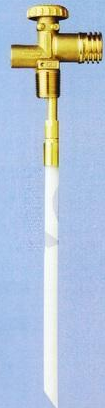
\includegraphics[height=5cm,width=5cm]{lot_valve}\label{lot_valve}}
		\subfloat[][SC Valve]{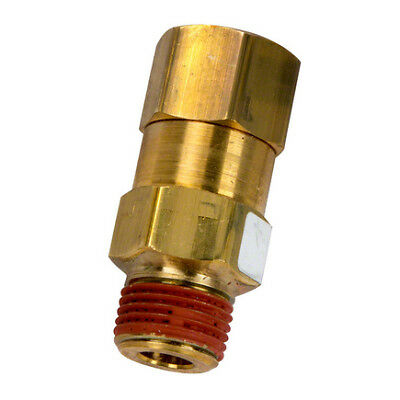
\includegraphics[height=5cm,width=5cm]{sc_valve}\label{sc_valve}}
		\caption{Types of valves attached to LPG cylinders}
		\label{lpg_valves}
	\end{figure}
	\begin{figure}[h]
		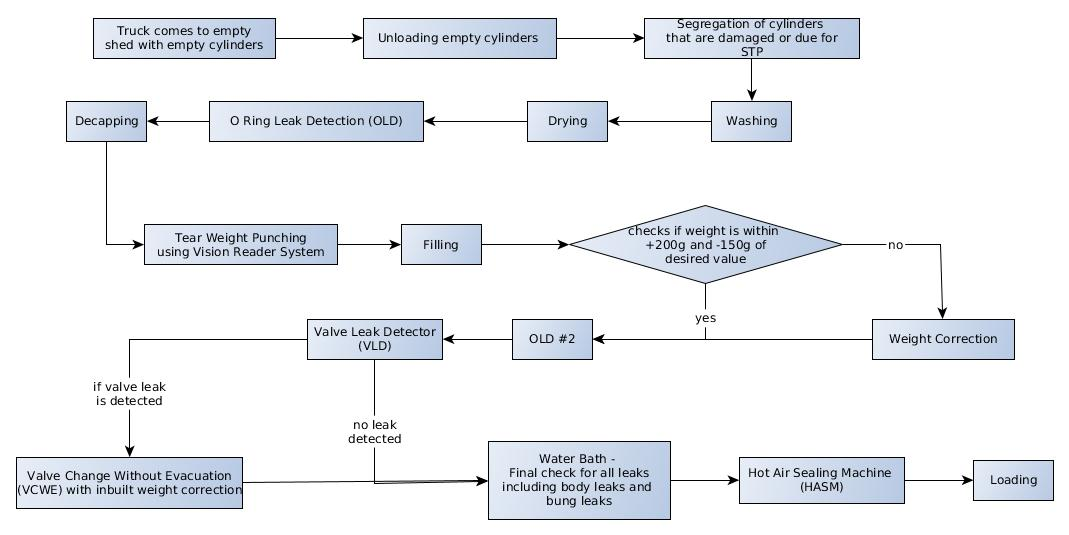
\includegraphics[width=\linewidth]{lpg_flow}
		\caption{LPG filling process flow}
		\label{lpg_flow}
	\end{figure}
		\begin{figure}[h]
		\centering
		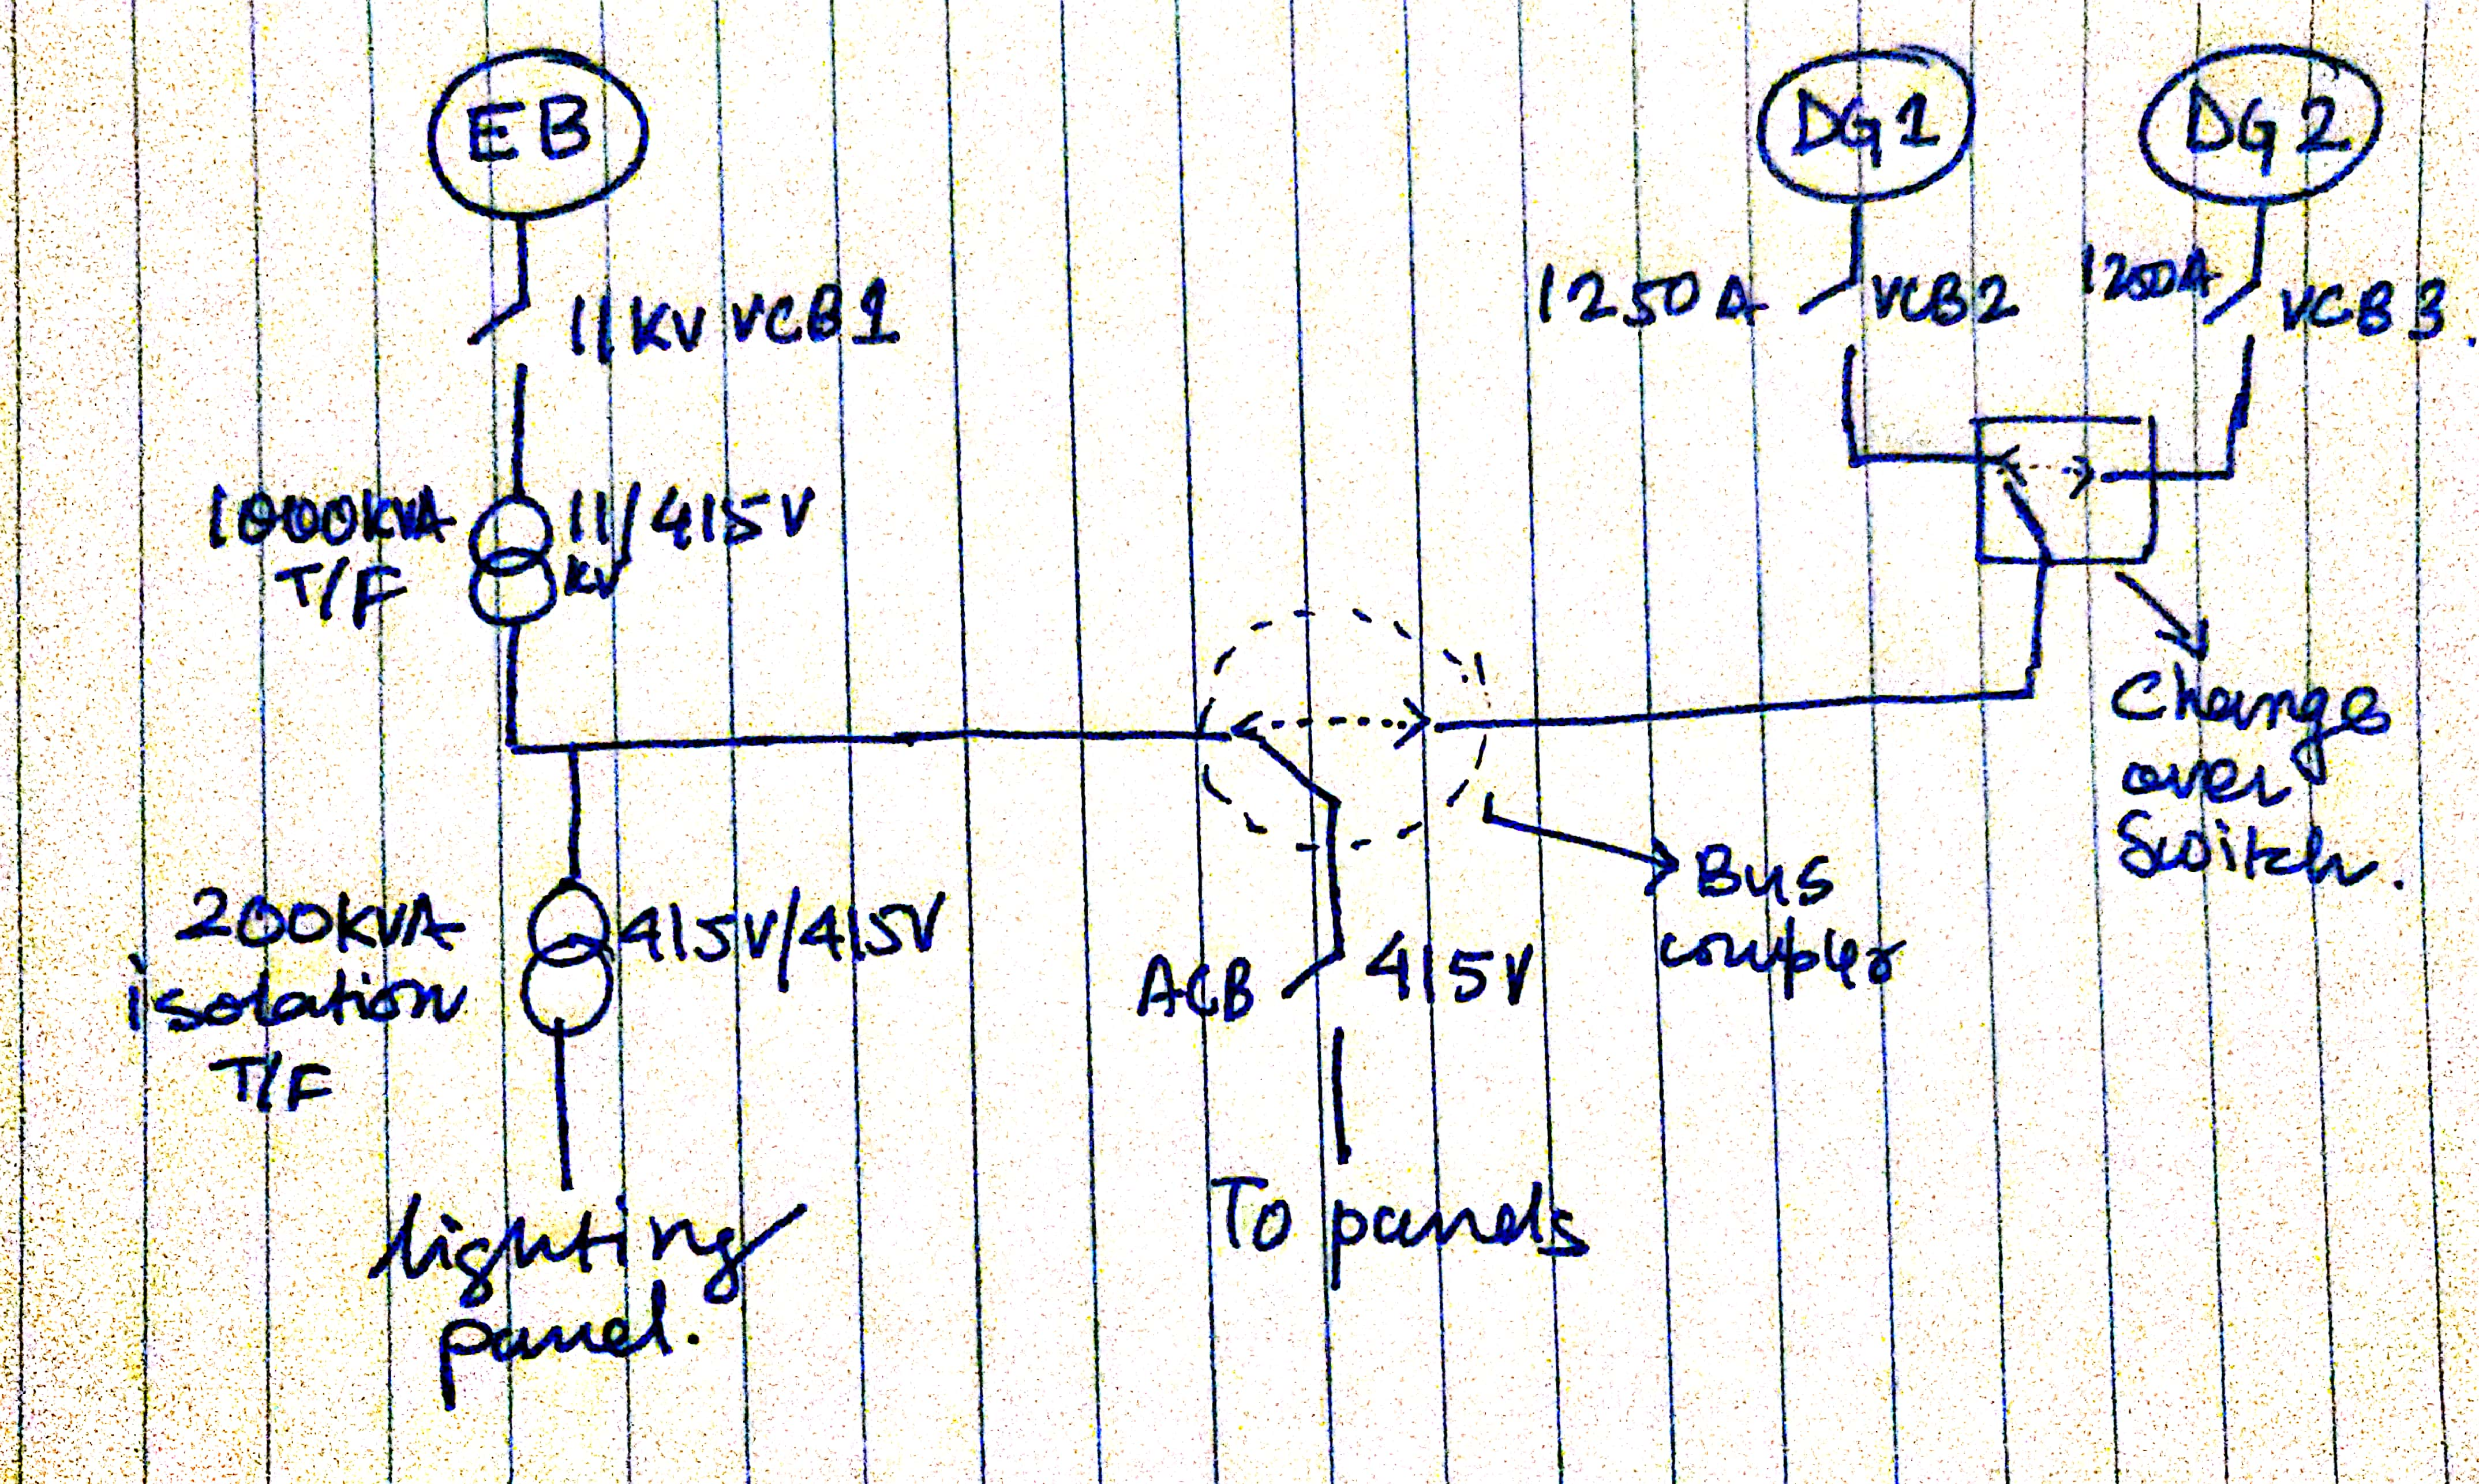
\includegraphics[width=\linewidth]{bp_singlelinediag}
		\caption{Basic single line diagram of a bottling plant electrical distribution system}
		\label{bp_singlelinediag}
	\end{figure}
	\begin{figure}[h]
		\centering
		\subfloat[][Schematic diagram of a Switch Fuse Unit]{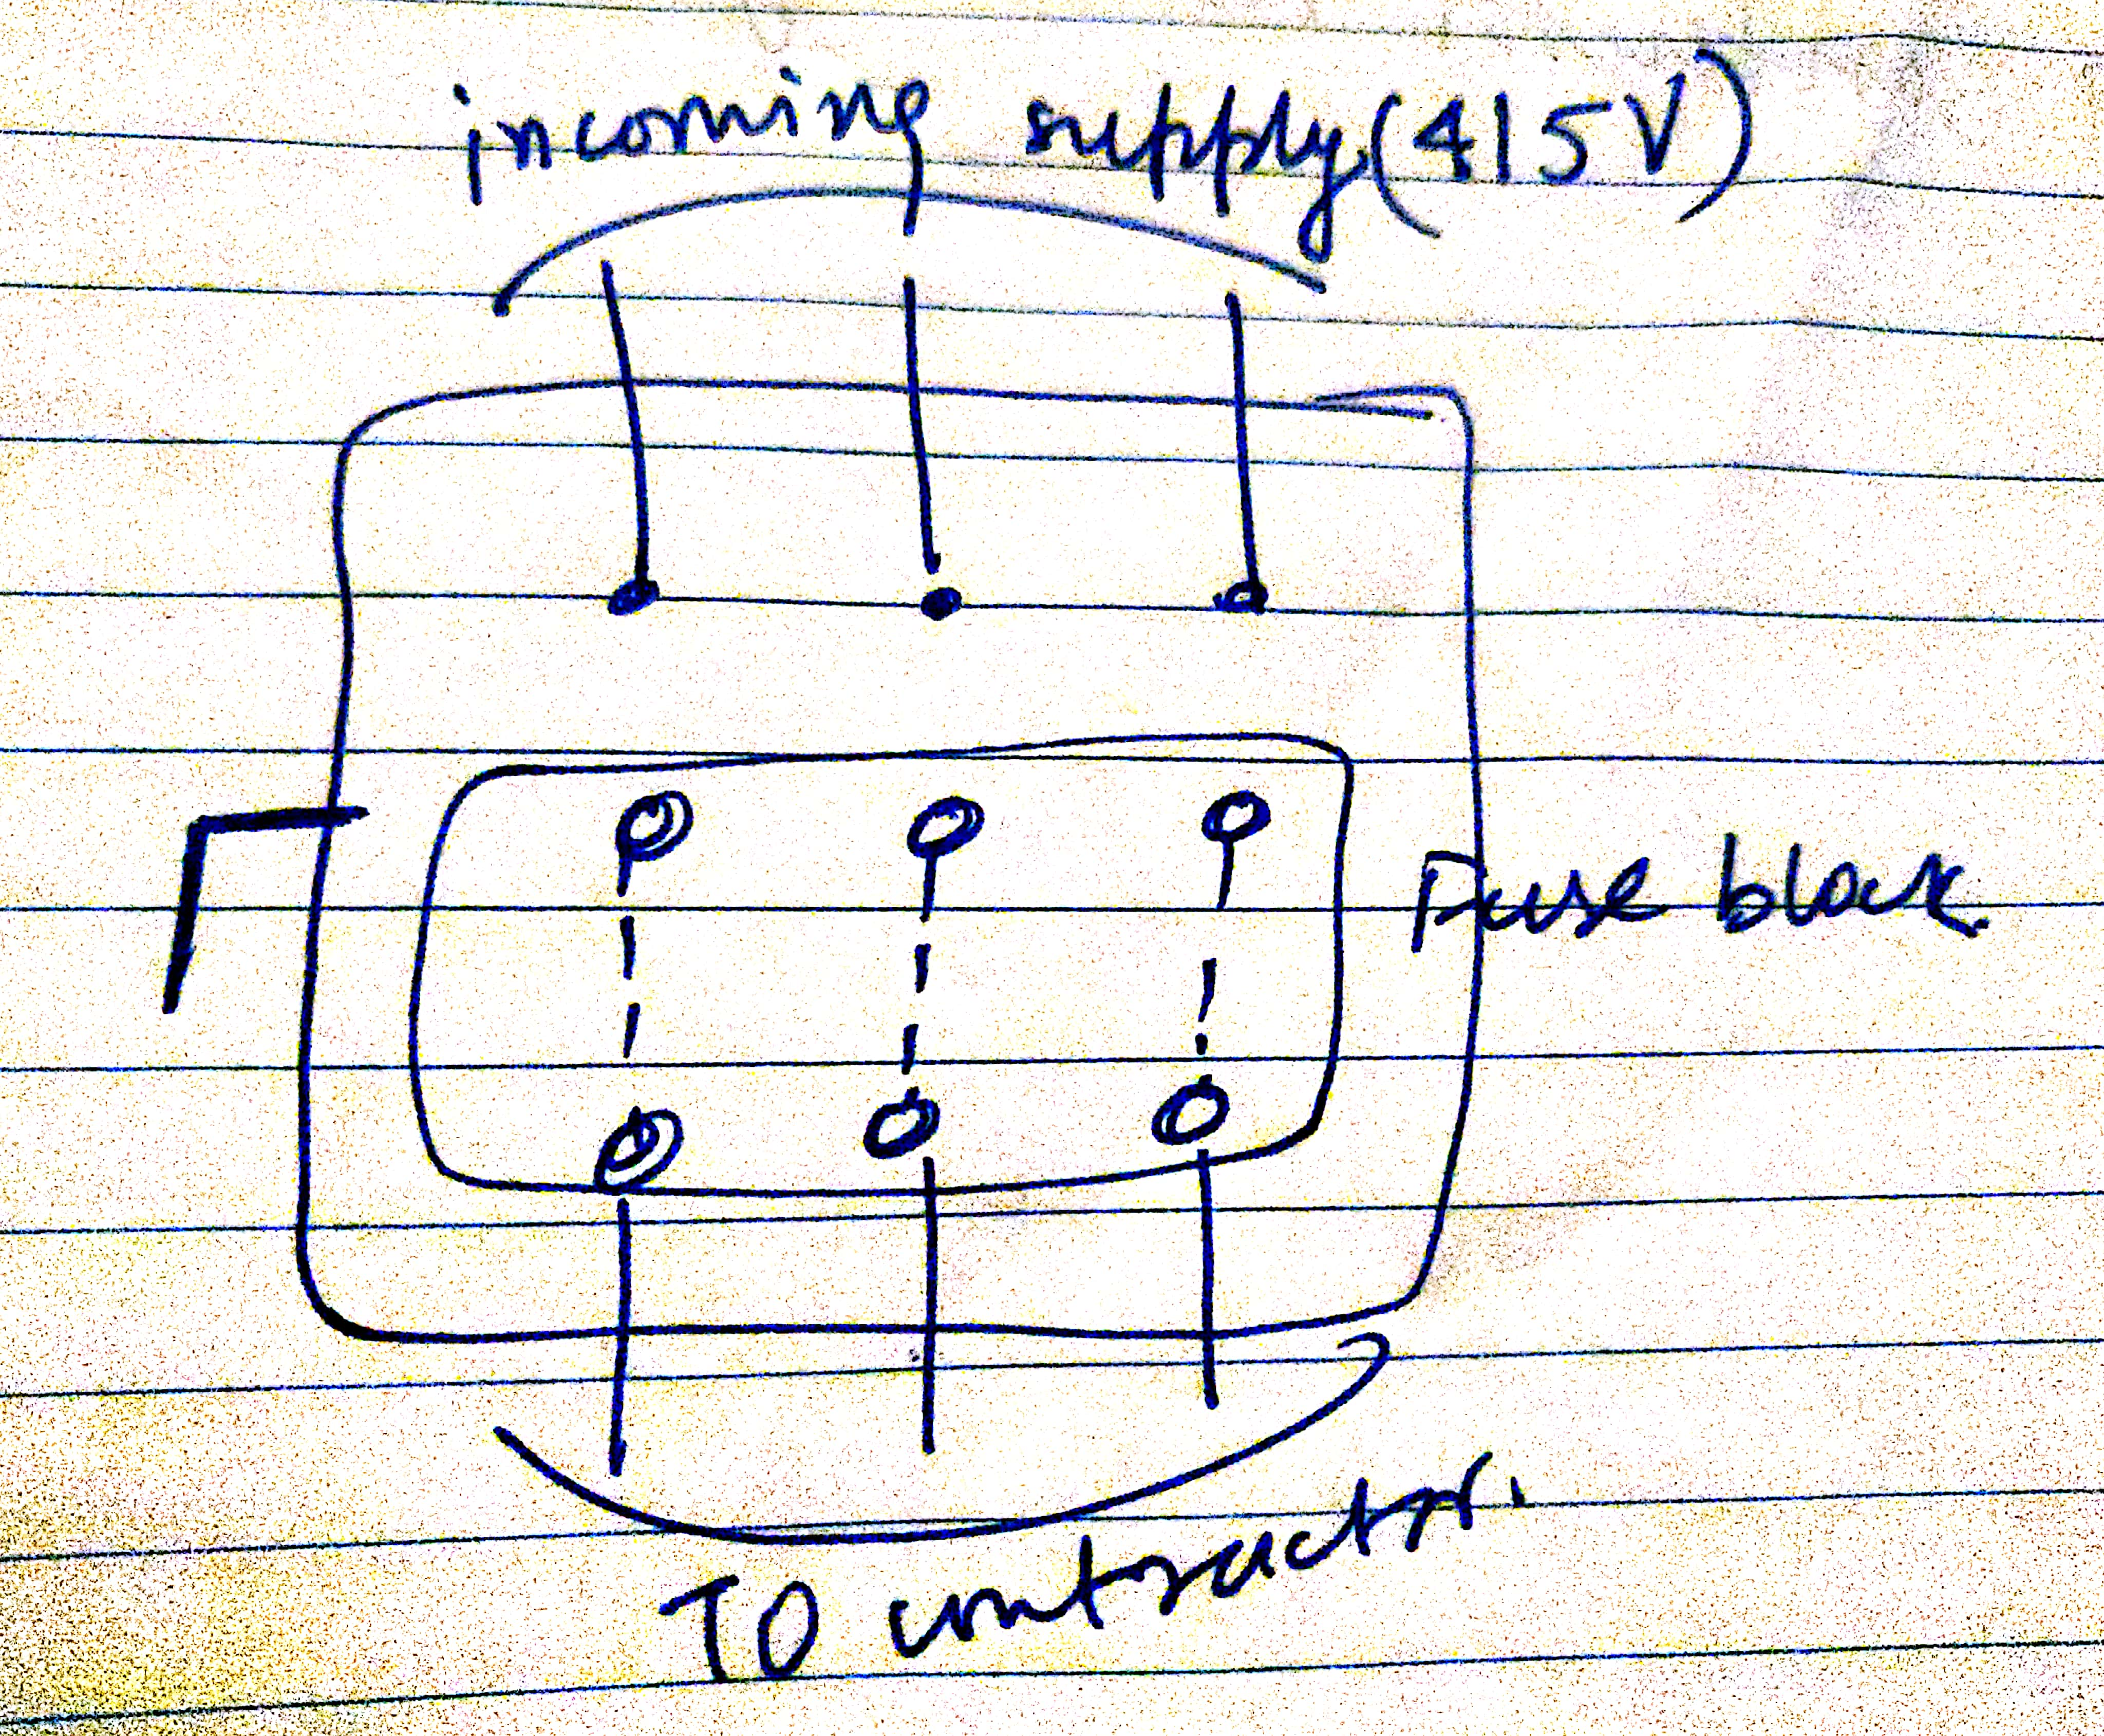
\includegraphics[width=0.5\linewidth]{sfu}\label{sfu}}
		\subfloat[][Inside view of a panel showing its safety features]{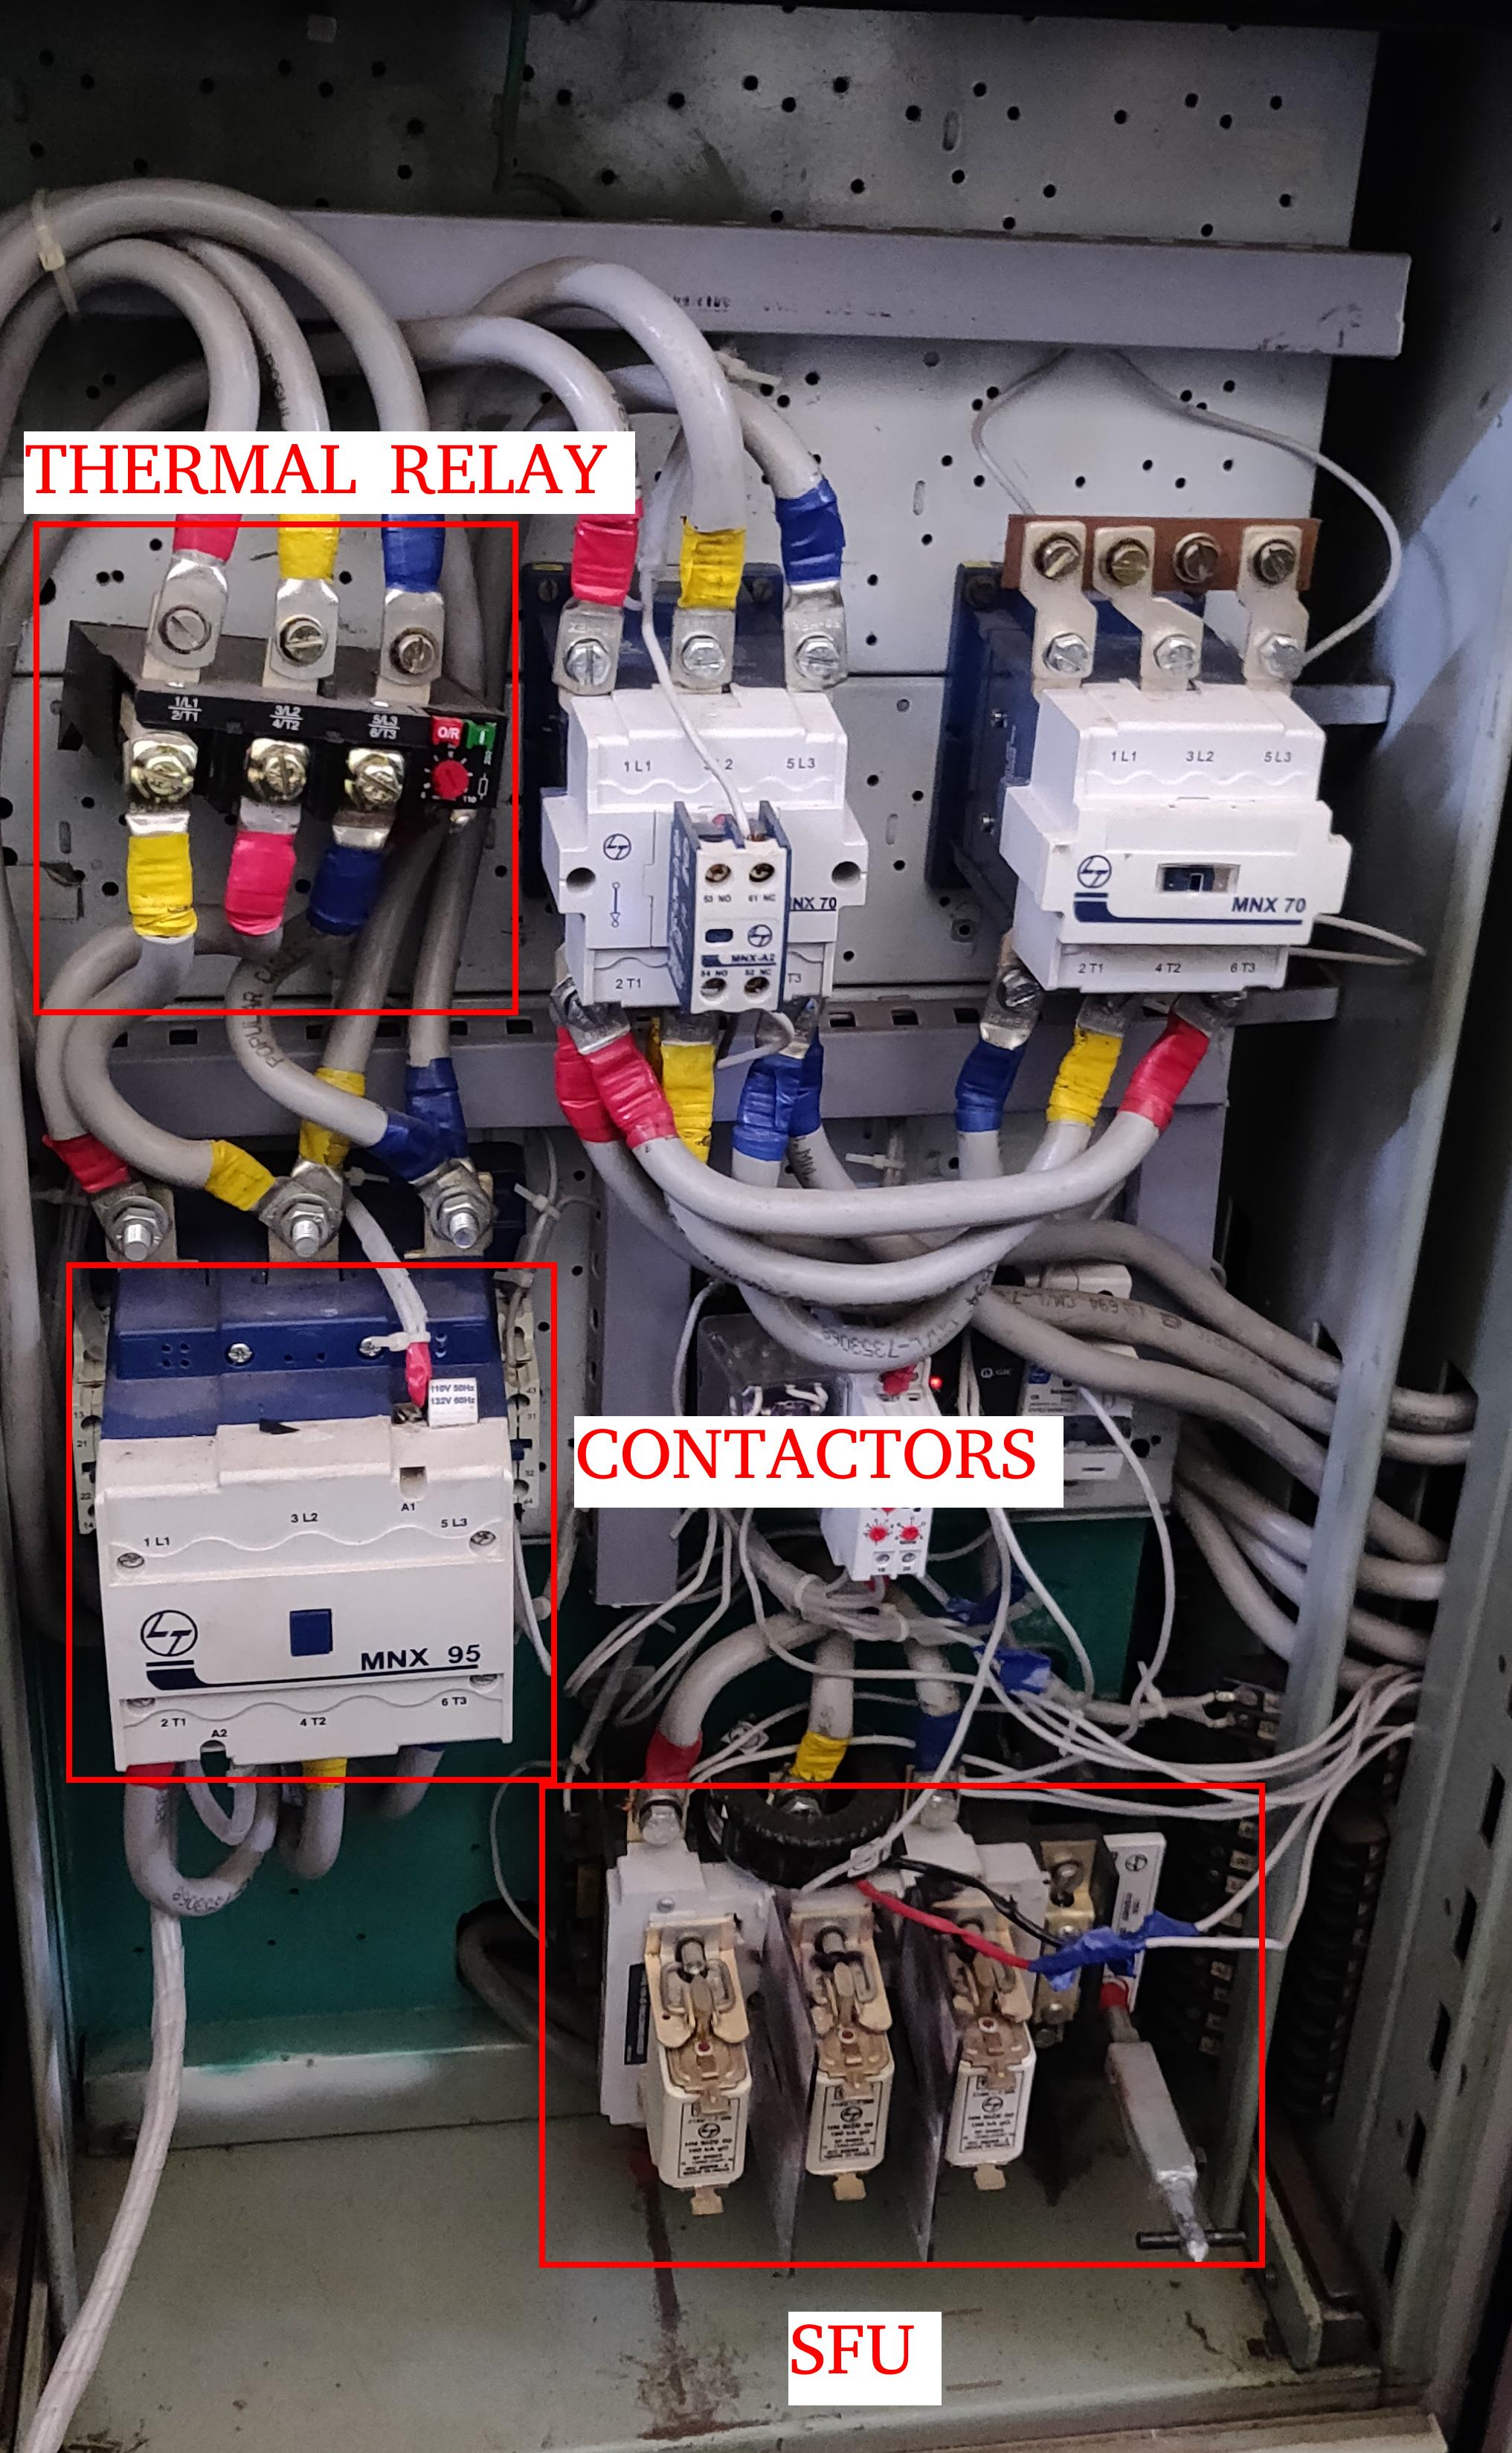
\includegraphics[height=10cm,width=0.5\linewidth]{inside_panel}\label{inside_panel}}
		\caption{Theoretical and real panel equipment protection apparatus}
		\label{bp_panel}
	\end{figure}
	\begin{figure}[h]
		\centering
		\subfloat[Schematic diagram of the dc power delivery system]{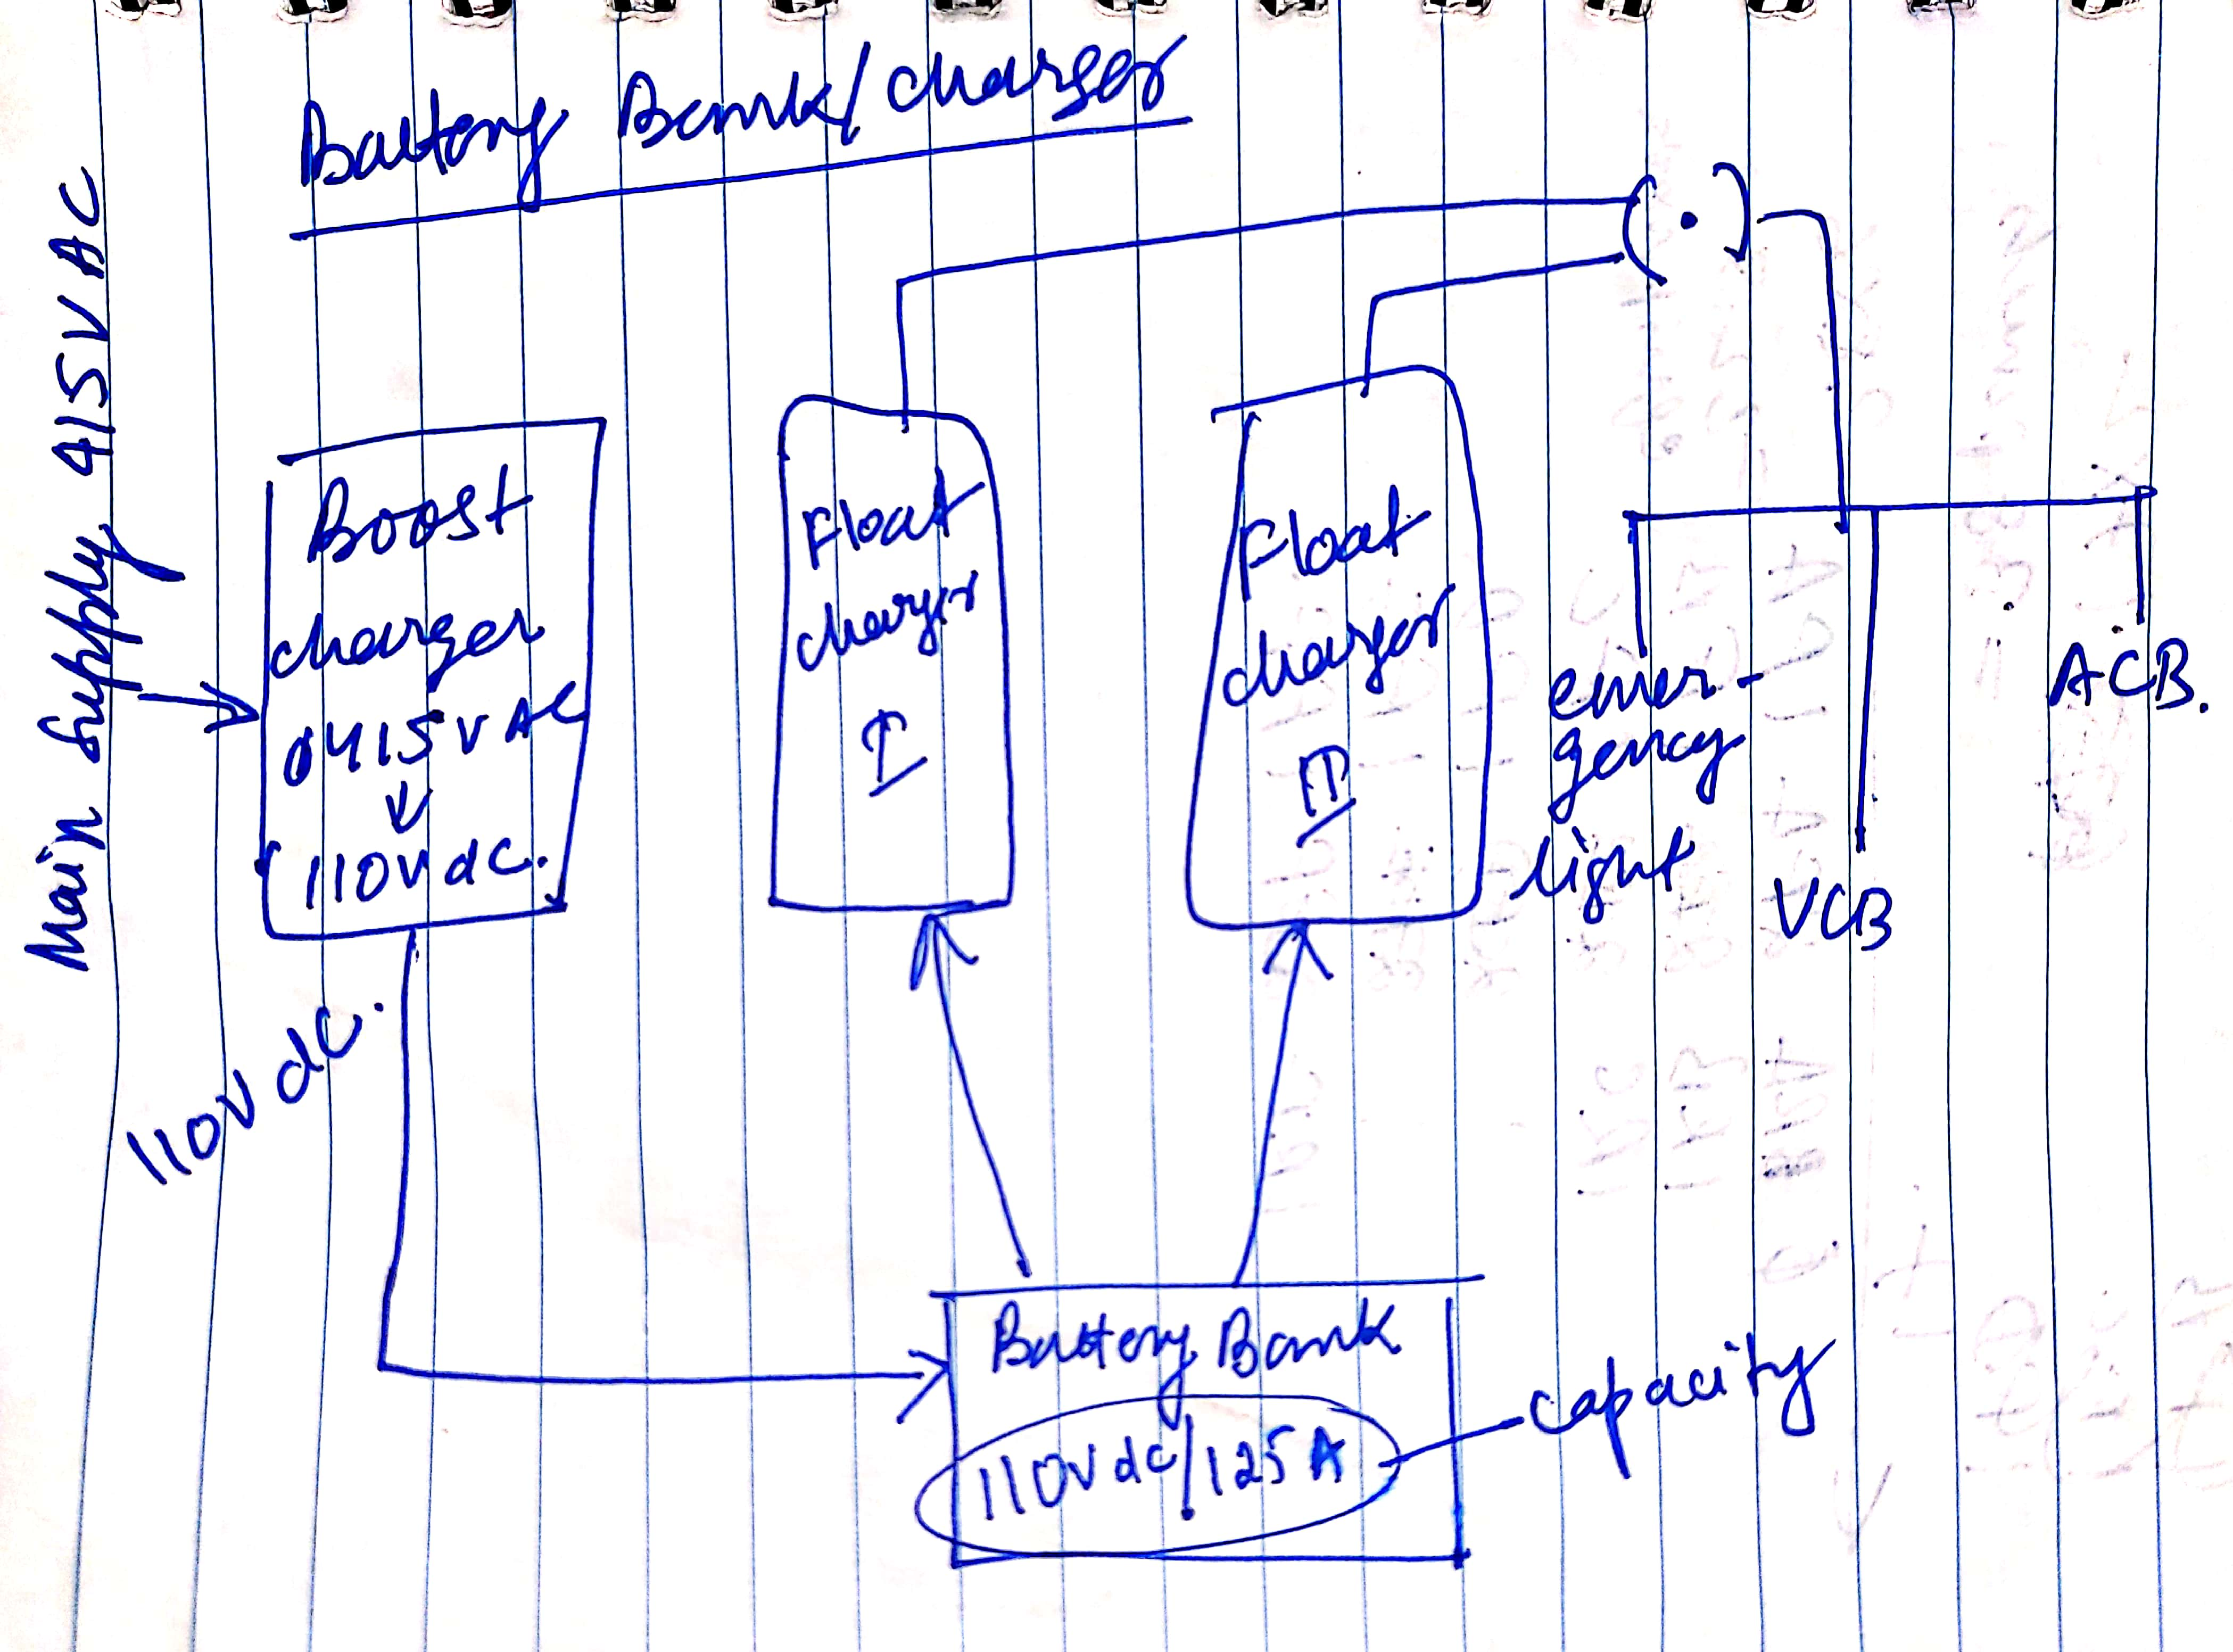
\includegraphics[width=0.5\linewidth]{dc_distribution}\label{dc_distribution}}
		\subfloat[Schematic diagram of the dc power delivery system]{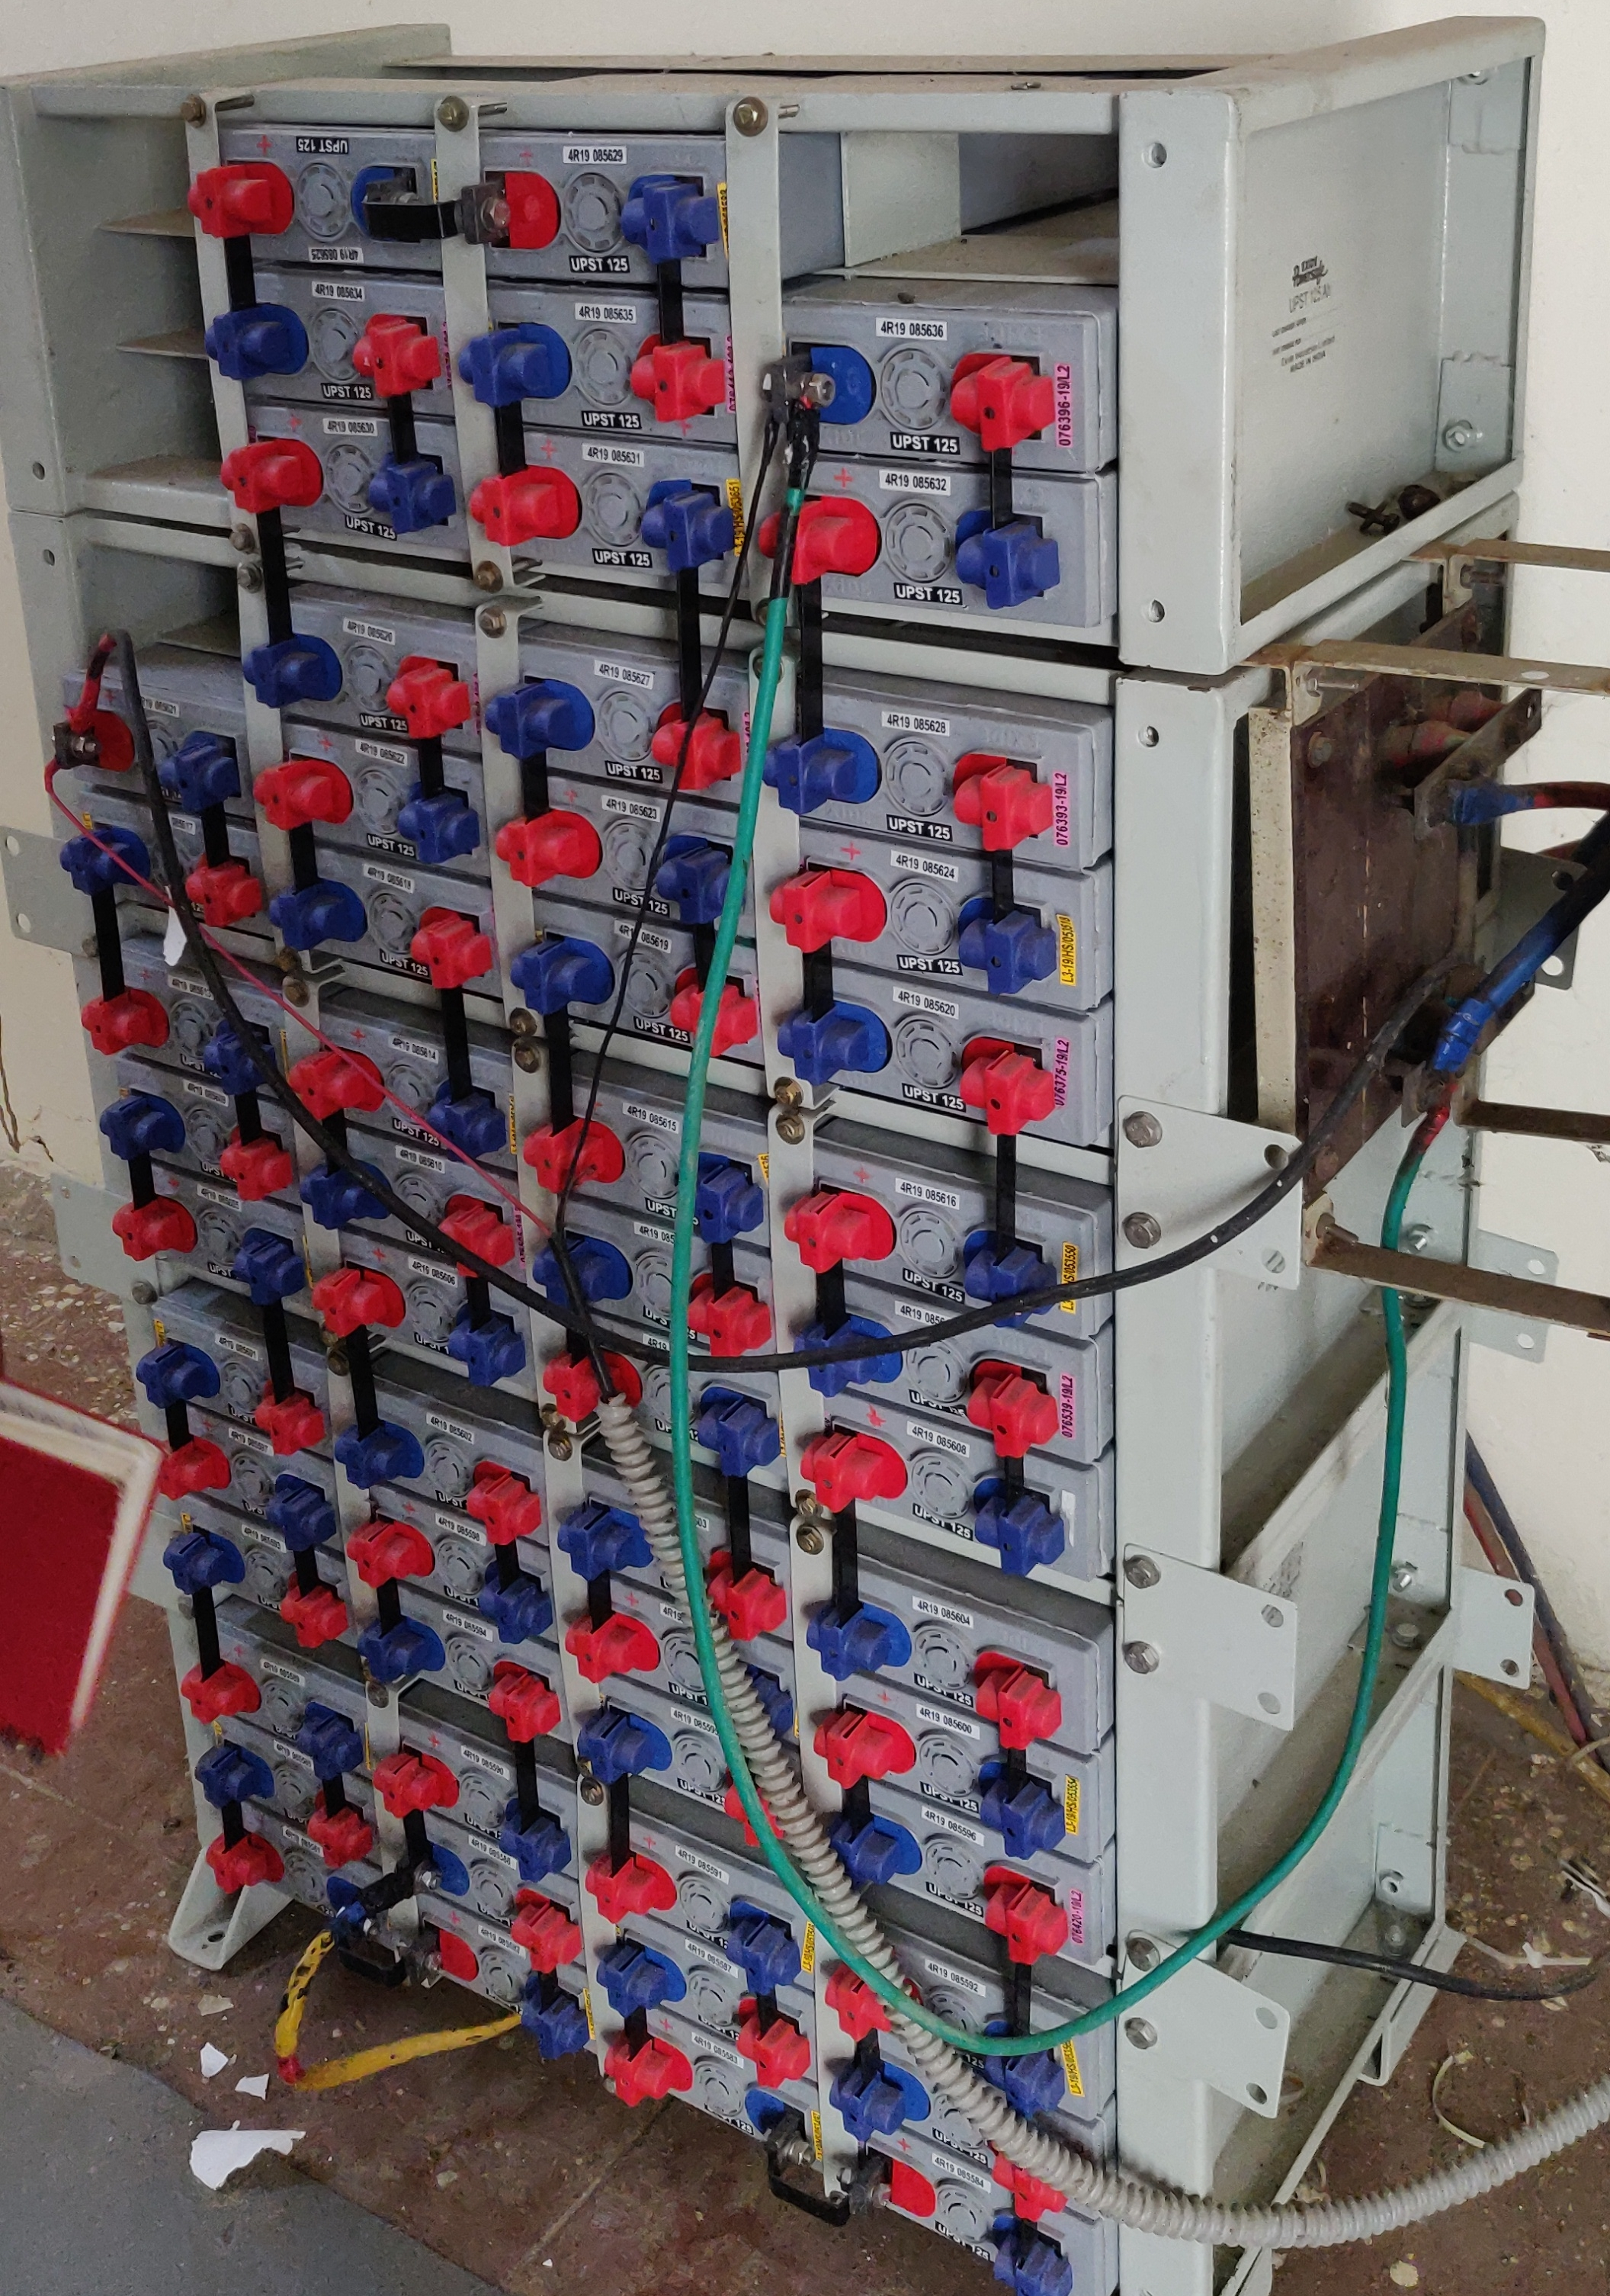
\includegraphics[height=10cm]{battery_pack_sanand}\label{battery_pack_sanand}}
		\caption{DC power delivery system}
		\label{dc_power_sanand}
	\end{figure}
	\begin{figure}[h]
		\centering
		\subfloat[][Neutral Earthing]{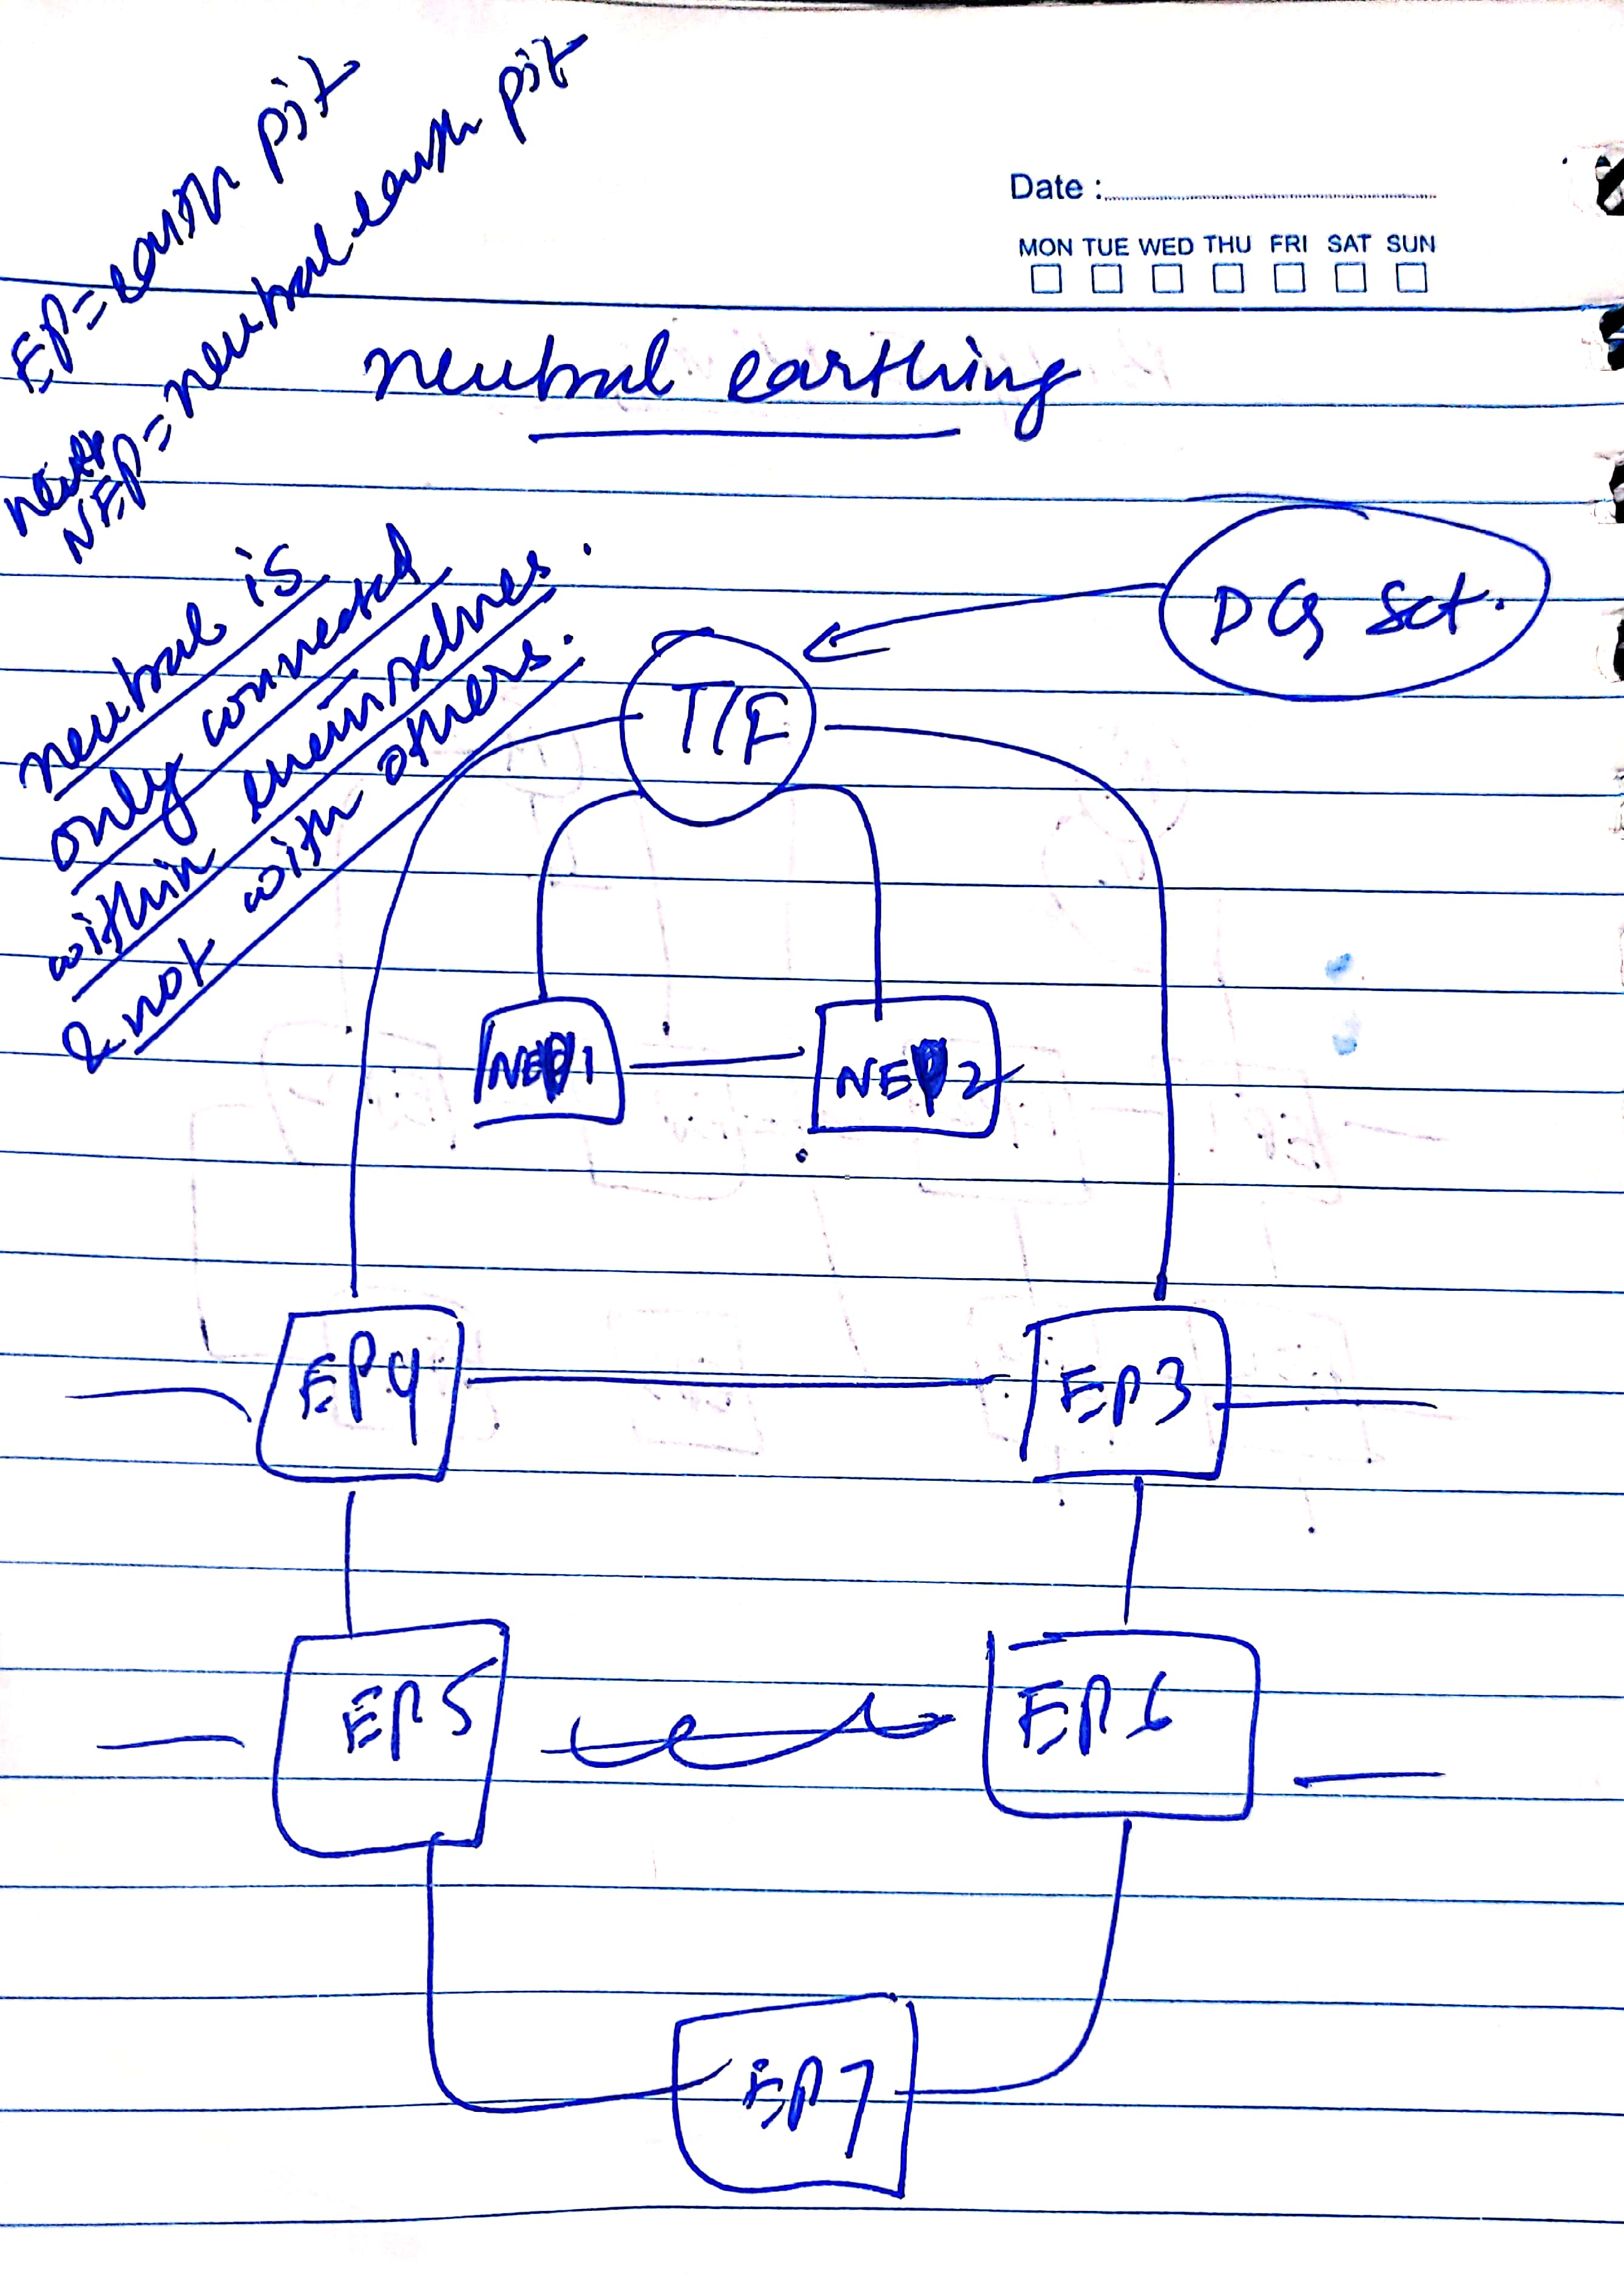
\includegraphics[height=10cm,width=0.33\linewidth]{neutral_earthing}\label{neutral_earthing}}
		\subfloat[][Lightning Earthing]{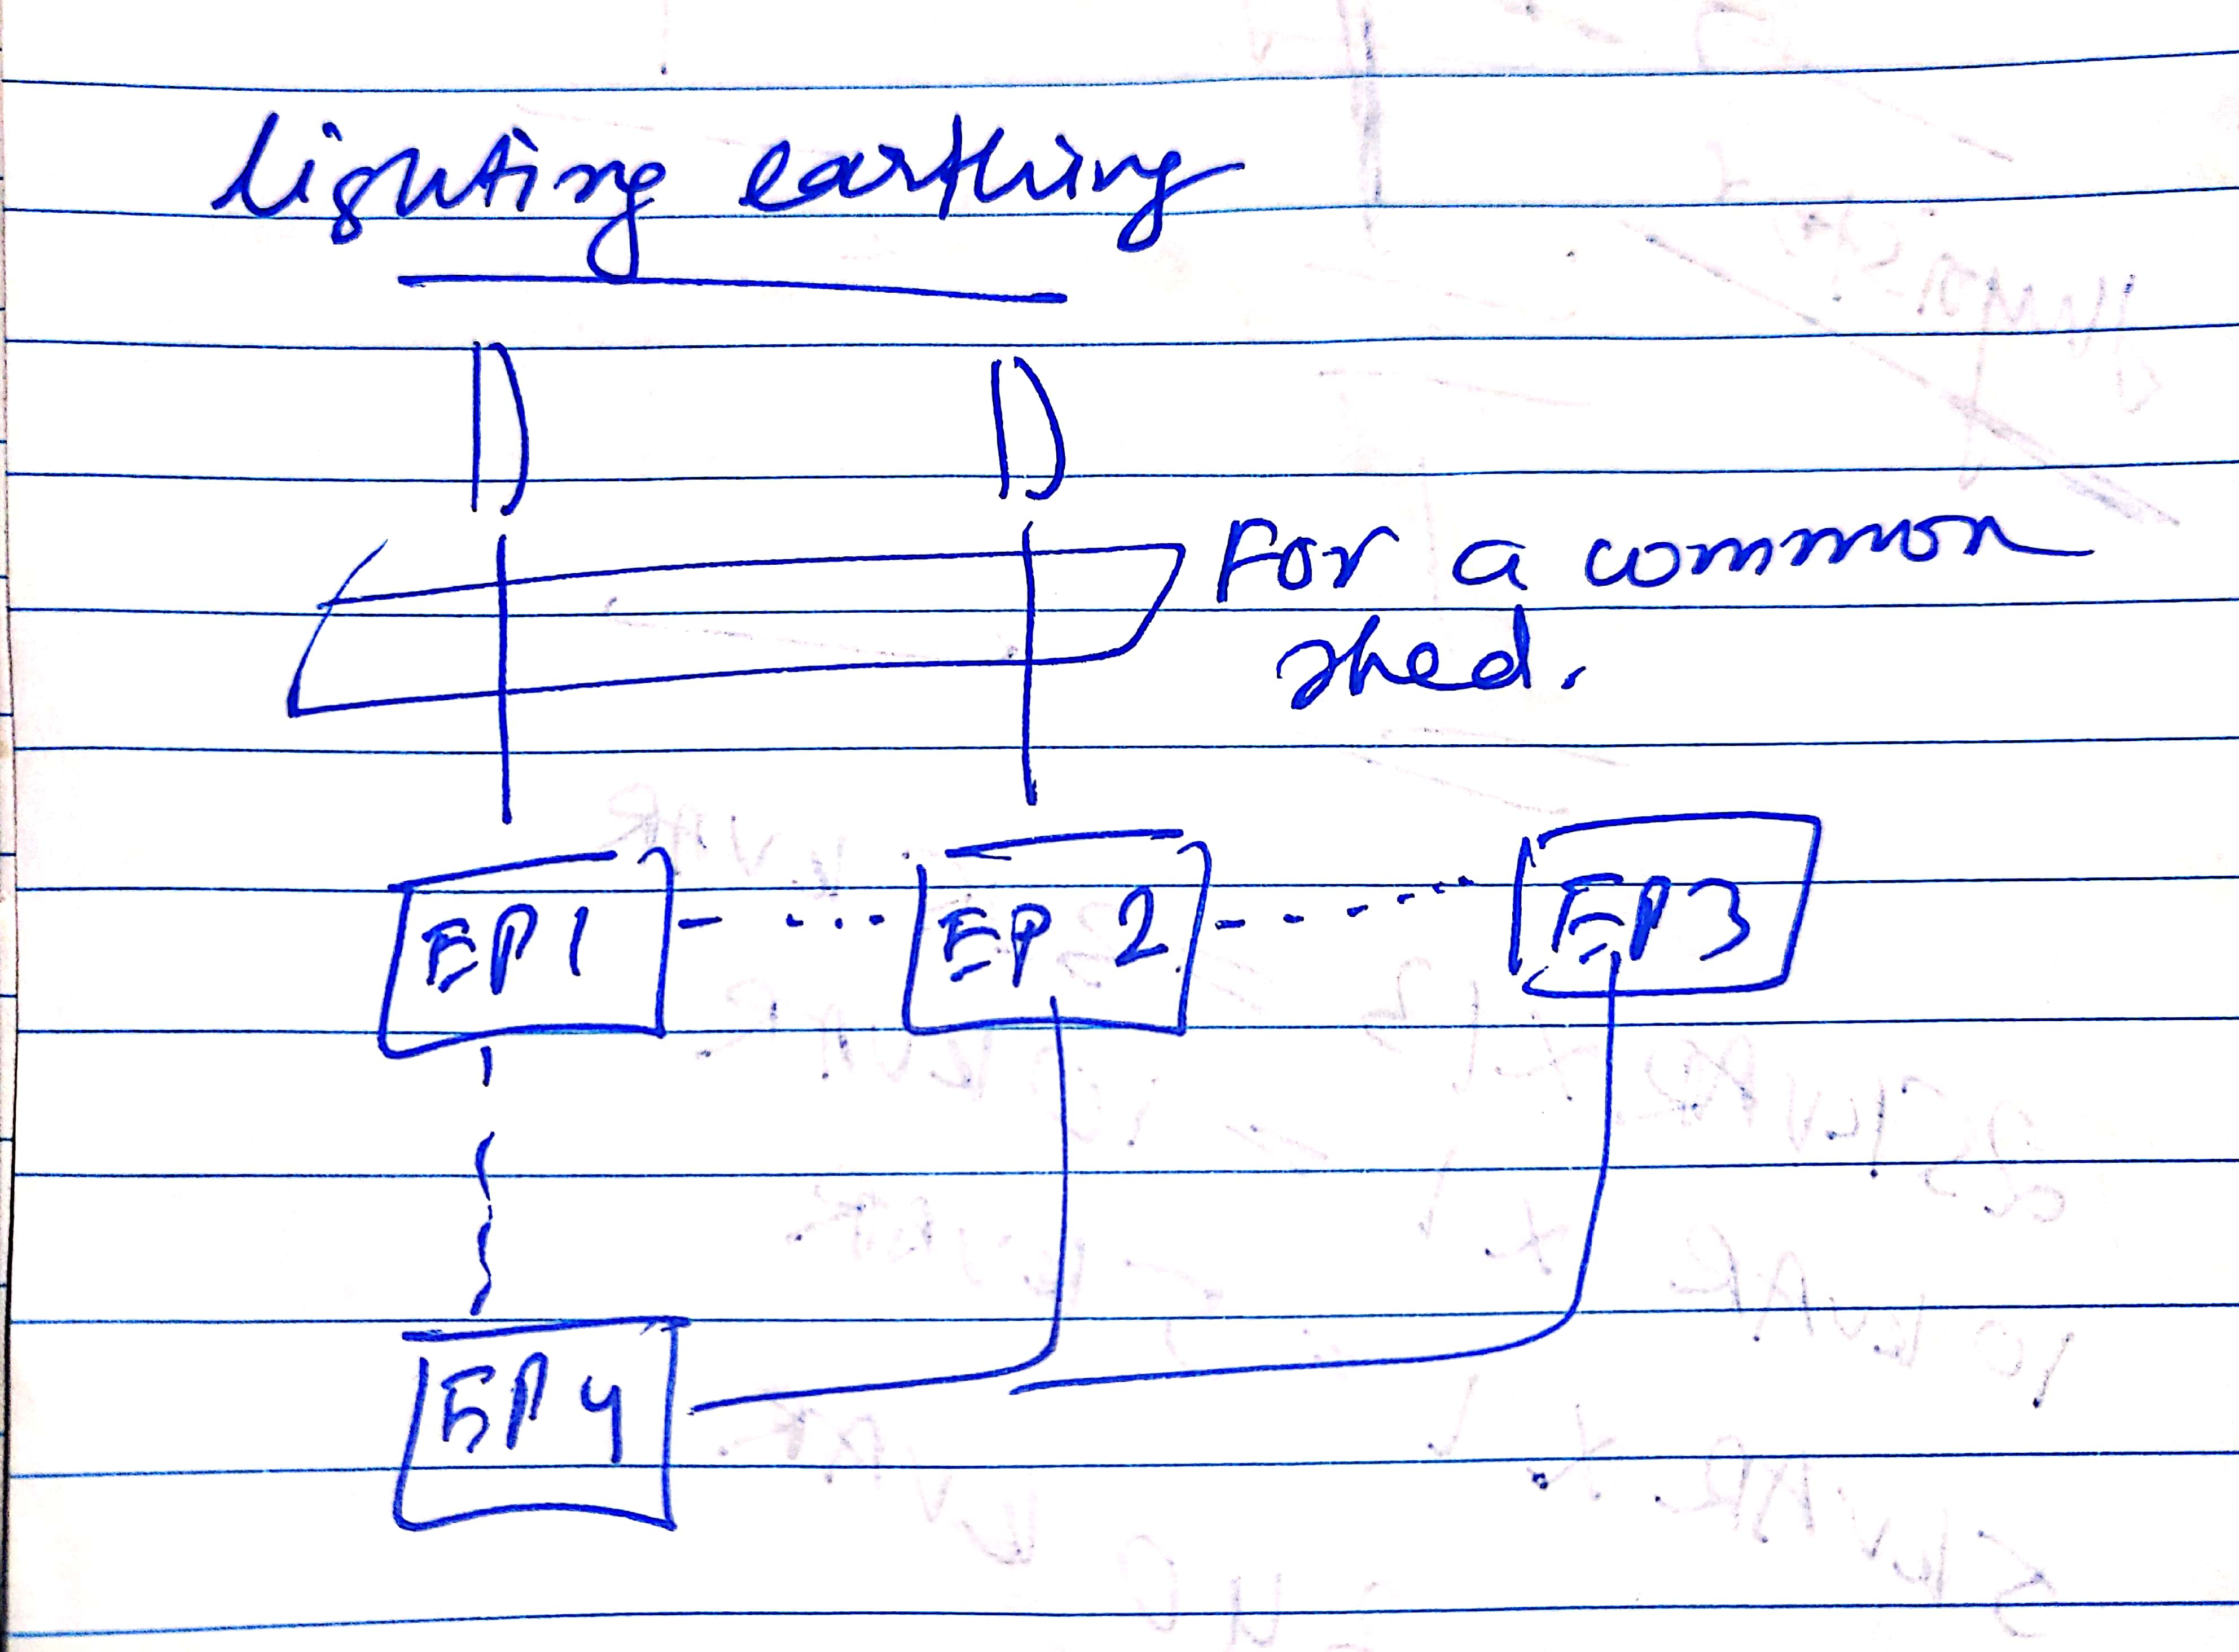
\includegraphics[height=10cm,width=0.33\linewidth]{lightning_earthing}\label{lightning_earthing}}
		\subfloat[][Body Earthing]{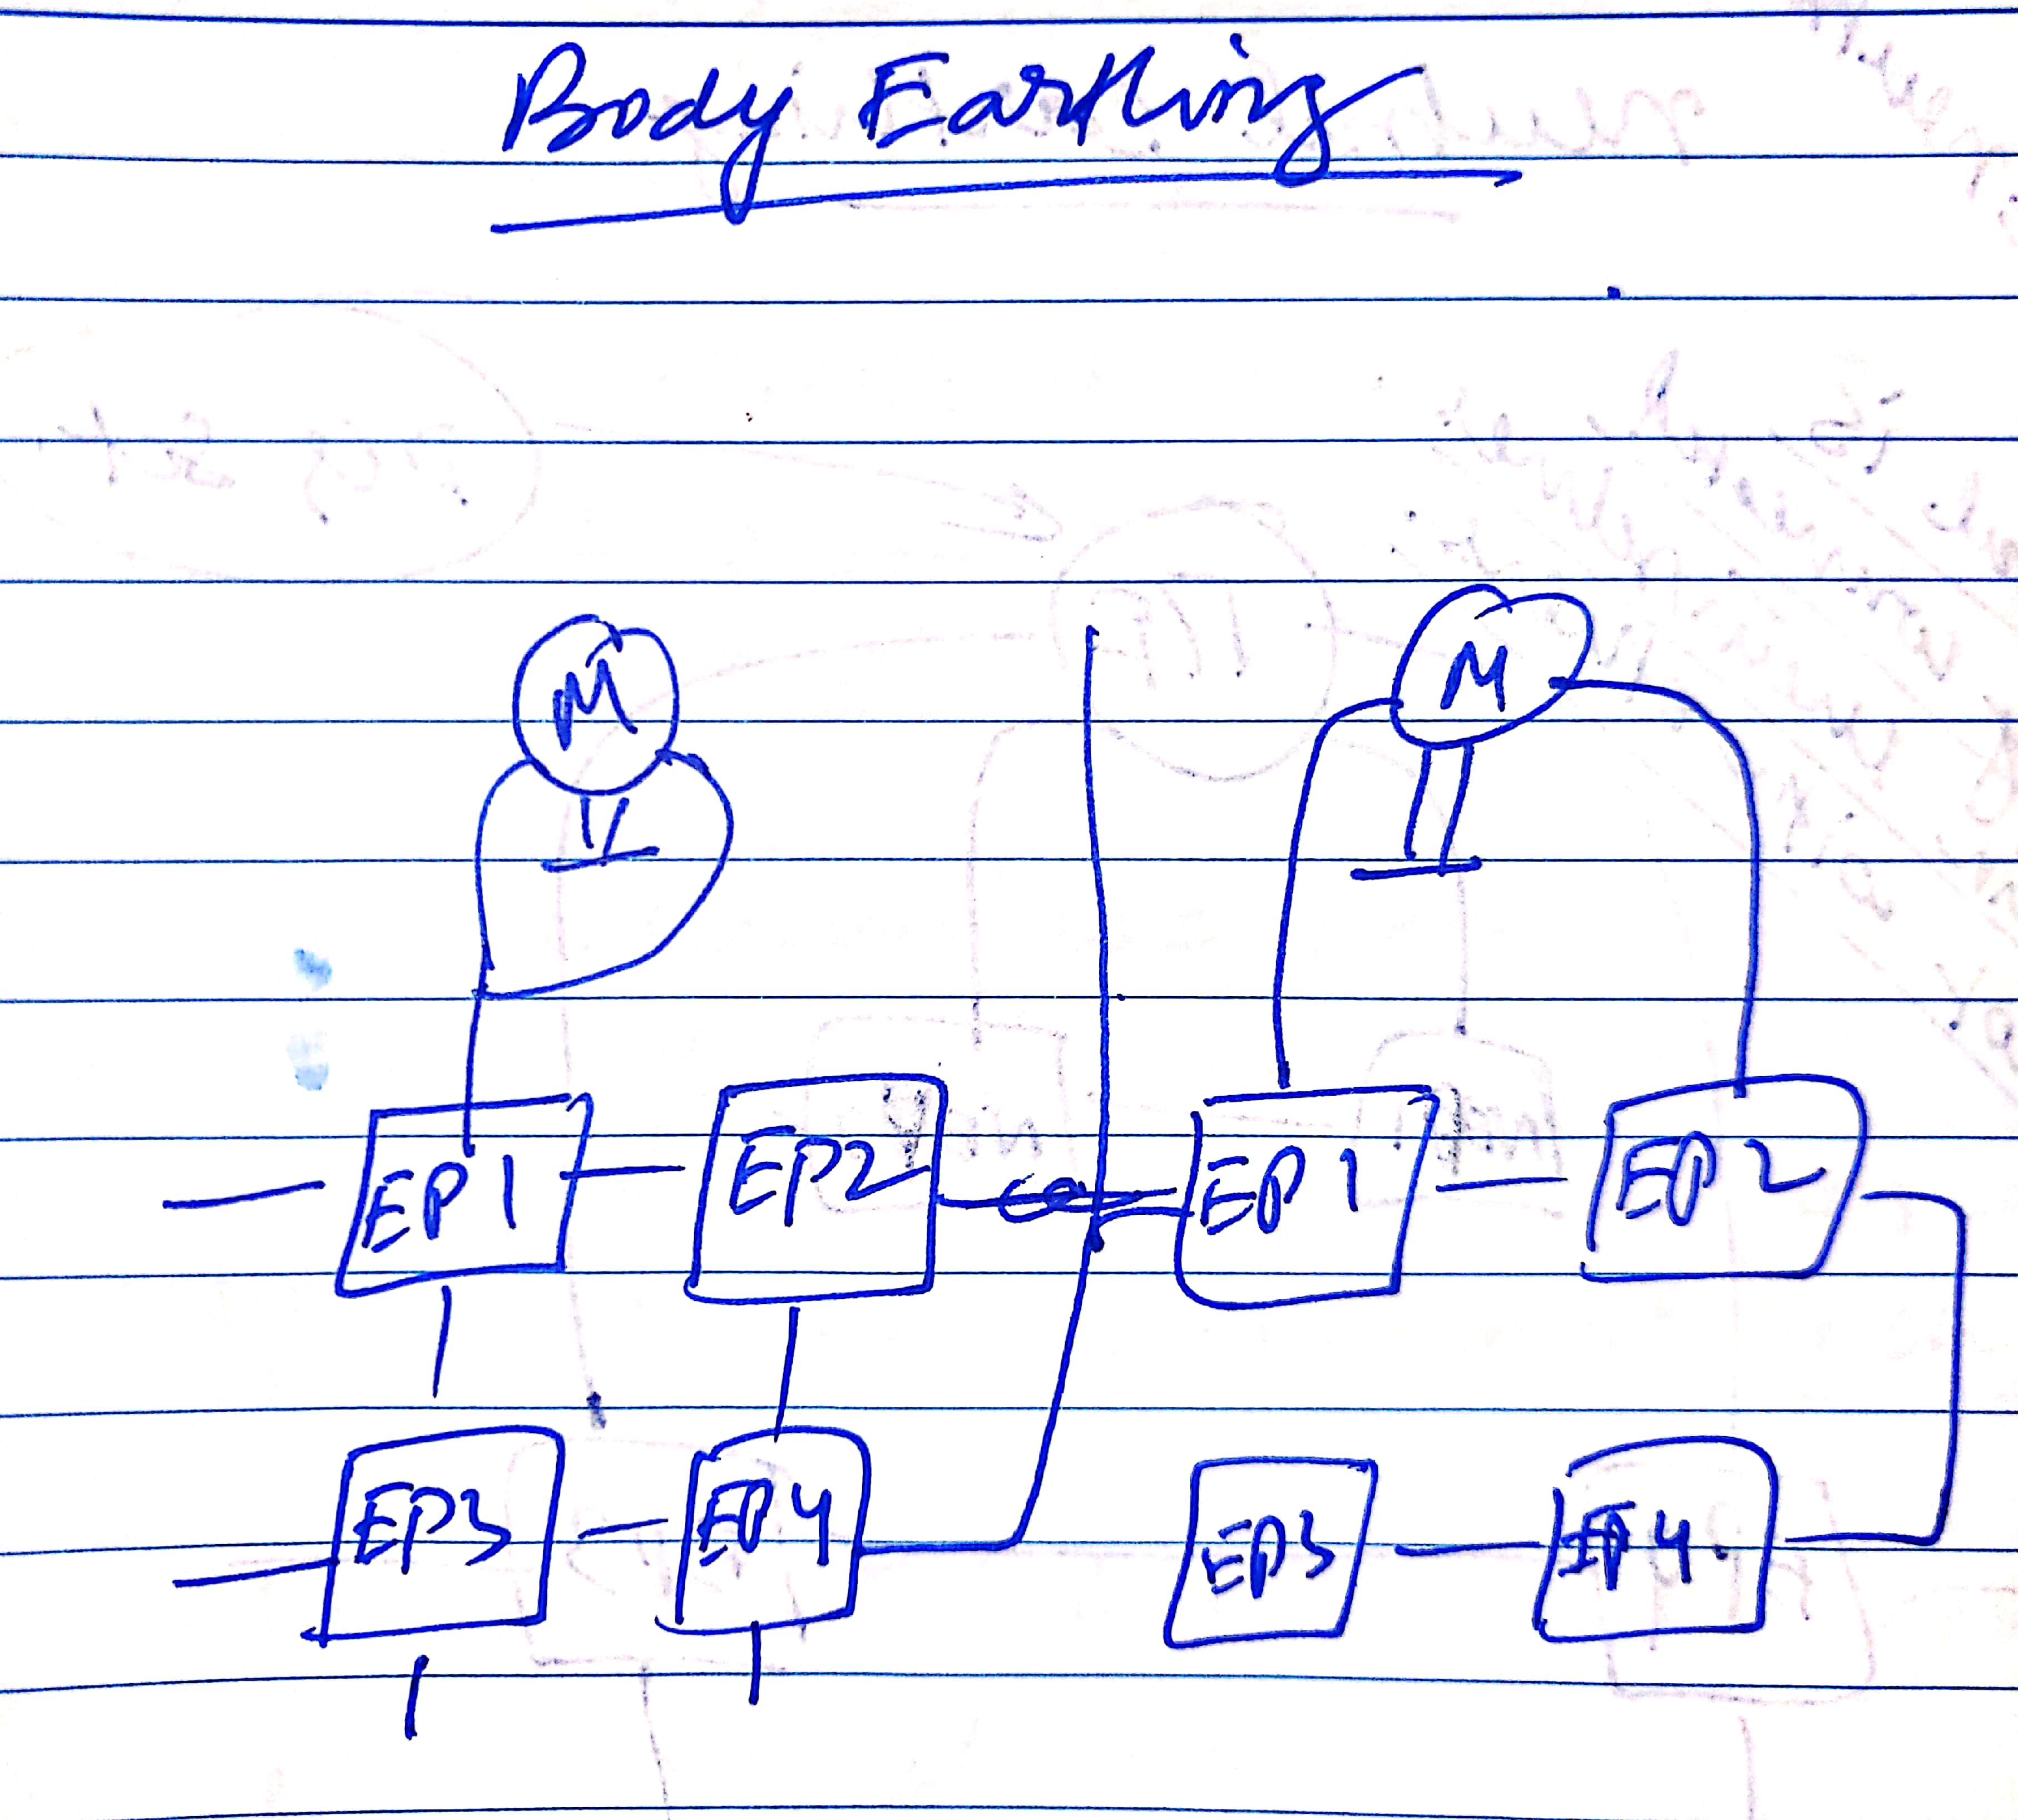
\includegraphics[height=10cm,width=0.33\linewidth]{body_earthing}\label{body_earthing}}
		\caption{Different types of earthing schemes}
		\label{bp_earthing}
	\end{figure}
	\begin{figure}[h]
		\centering
		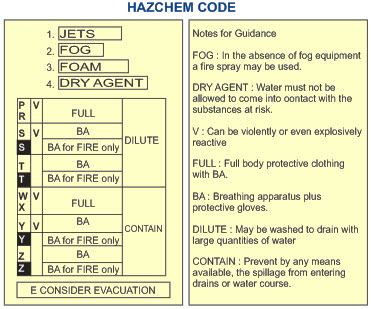
\includegraphics[width=0.5\linewidth]{hazchem}
		\caption{Hazchem decoded (BA=Breathing Apparatus)}
		\label{hazchem}
	\end{figure}
\end{document}